%% This is samplepaper.tex, a sample chapter demonstrating the
%% LLNCS macro package for Springer Computer Science proceedings;
%% Version 2.21 of 2022/01/12

\documentclass[runningheads]{llncs}
%
\usepackage{inputenc}
\usepackage[T1]{fontenc}

\usepackage{amsmath,amssymb,amsfonts}
% \usepackage{times}
\usepackage{listings}
\usepackage{float}
\usepackage{wrapfig,caption,subcaption}
%\usepackage{romannum}
\usepackage{paracol}
\usepackage{graphicx}
\usepackage{rotating}
\usepackage{textcomp}
\usepackage{xcolor}
\usepackage{tabularx}
\usepackage{array}
\usepackage{txfonts}
\usepackage{mathtools}
\usepackage{pmboxdraw}
\def\nbR{\mathbb{R}}

% special environments
\usepackage{multicol}
\usepackage{multirow}
\usepackage[linesnumbered,lined,boxed,commentsnumbered]{algorithm2e}
\usepackage{paralist}
\usepackage[inline]{enumitem}
\usepackage{mathpartir} % SOS rules
\usepackage{comment}

% TikZ
\usepackage{tikz}
\usepackage{verbatim}
\usetikzlibrary{patterns}
\usetikzlibrary{shapes.callouts}
\usetikzlibrary{arrows,decorations.pathmorphing,backgrounds,fit,positioning,shapes.symbols,chains}
\usetikzlibrary{shapes,arrows.meta,calc,fit,shapes.multipart,positioning}

\newenvironment{textlist}{\begin{enumerate*}[label=(\emph{\roman*})]}{\end{enumerate*}}

\newenvironment{rqs}{\begin{enumerate}[label=\textbf{RQ\arabic*}]}{\end{enumerate}}

% branching in TeX commands
\usepackage{ifthen}


% Abbreviations
\usepackage[acronym,prefix]{glossaries-extra}
\setabbreviationstyle[acronym]{long-short}
\newacronym{bip}{BIP}{Behaviour-Interaction-Priority}
\newacronym{dag}{DAG}{Directed Acyclic Graph}
\newacronym{drbip}{DR-BIP}{Dynamic Reconfigurable BIP}
\newacronym[prefixfirst={a~},prefix={an\space}]{sos}{SOS}{Structural Operational Semantics}
\newacronym[prefixfirst={a~},prefix={an\space}]{lts}{LTS}{Labelled Transition System}
\newacronym[prefixfirst={a~},prefix={an\space}]{fol}{FOL}{First Order Logics}
\newacronym{cps}{CPS}{Cyber-Physical System}

% --- PDF SUPPORT ----------------------

\usepackage{hyperref}  % import as last package
\usepackage[capitalise]{cleveref}[2012/02/15]  % import after hyperref
\crefformat{footnote}{#2\footnotemark[#1]#3}

%%%%%%%%%%%%%%%%%%%%%%%%%%%%%%%%%%%%%%%%%%%%%%%%%%%%%%%%%%%%


\newcommand{\secn}[1]{\cref{secn:#1}}
%\newcommand{\secn}[1]{Sect.~\ref{secn:#1}}
%\newcommand{\fig}[1]{\figurename~\ref{fig:#1}}
\newcommand{\fig}[1]{\cref{fig:#1}}
\newcommand{\figs}[2]{Figures~\ref{fig:#1} and \ref{fig:#2}}
\newcommand{\eq}[1]{(\ref{eq:#1})}
\newcommand{\eqs}[2]{(\ref{eq:#1}) and (\ref{eq:#2})}
\newcommand{\hyp}[1]{(\ref{hyp:#1})}
\newcommand{\defn}[1]{Def.~\ref{defn:#1}}
\newcommand{\prop}[1]{Prop.~\ref{prop:#1}}
\newcommand{\Prop}[1]{Proposition~\ref{prop:#1}}
\newcommand{\thm}[1]{\cref{thm:#1}}
\newcommand{\ex}[1]{\cref{ex:#1}}
\newcommand{\exs}[2]{Examples~\ref{ex:#1} and \ref{ex:#2}}

\newcommand{\mdash}[1][]{{#1}---{#1}}
\newcommand{\eg}[1][\@ ]{e.g.{#1}}
\newcommand{\Eg}[1][\@ ]{E.g.{#1}}
\newcommand{\ie}[1][\@ ]{i.e.{#1}}
\newcommand{\viz}[1][\@ ]{viz.{#1}}
\newcommand{\etc}[1][\@ ]{etc.{#1}}
\newcommand{\resp}[1][\@ ]{resp.{#1}}
\newcommand{\cf}{cf.\@ }
\newcommand{\vs}{vs.\@ }
\newcommand{\wrt}{w.r.t.\@ }

\newcommand{\sB}{\mathbb{B}}

\newcommand{\true}{\mathit{true}}
\newcommand{\false}{\mathit{false}}

\newcommand{\bydef}{\mathbin{\stackrel{\scriptscriptstyle\mathit{def}}{=}}}

\newcommand{\setdef}[2]{\{#1\,|\,#2\}}
\newcommand{\bsetdef}[2]{\bigl\{#1\,\bigr.\bigl|\,#2\bigr\}}
\newcommand{\Bsetdef}[2]{\left\{\left.#1\,\right|\,#2\right\}}
\newcommand{\BRsetdef}[2]{\left\{#1\,\left|\,#2\right.\right\}}

\newcommand{\goesto}[2][]{\xrightarrow[#1]{#2}}

\newcommand{\condition}{\mathit{cnd}}


\newcommand{\code}[1]{\mathtt{#1}}
\newcommand{\nodename}[1]{\texttt{#1}}

\DeclareMathOperator{\dom}{dom}
\newcommand{\domain}[1]{\dom(#1)}
\newcommand{\abstracts}[1][]{\sqsubseteq\ifx#1\relax\else^{#1}\fi}
\newcommand{\refines}[1][]{\sqsupseteq\ifx#1\relax\else^{#1}\fi}
\newcommand{\isrefinedby}{\abstracts}
\newcommand{\issimulatedby}{\abstracts}

\newcommand{\assembly}[1][]{A\ifx#1\relax\else^{#1}\fi}
\newcommand{\motif}[1][]{M\ifx#1\relax\else^{#1}\fi}
\newcommand{\interface}[1][]{I\ifx#1\relax\else^{#1}\fi}
\newcommand{\map}[1][]{\mu\ifx#1\relax\else^{#1}\fi}
\newcommand{\predicates}[1][]{\mathcal{P}\ifx#1\relax\else^{#1}\fi}
\newcommand{\vertices}[1][]{V\ifx#1\relax\else^{#1}\fi}
\newcommand{\edges}[1][]{E\ifx#1\relax\else^{#1}\fi}
\newcommand{\nodes}[1][]{N\ifx#1\relax\else^{#1}\fi}
\newcommand{\data}[1][]{D\ifx#1\relax\else^{#1}\fi}
\newcommand{\ports}[1][]{P\ifx#1\relax\else^{#1}\fi}
\newcommand{\action}[1][]{a\ifx#1\relax\else^{#1}\fi}
\newcommand{\actionat}[2]{#2@#1}
\newcommand{\actionuniverse}[1][]{\mathit{Act}\ifx#1\relax\else^{#1}\fi}
\newcommand{\actions}[1][]{A\ifx\relax#1\relax\else^{#1}\fi}
\newcommand{\interaction}[1][]{\overline{\action}\ifx#1\relax\else^{#1}\fi}
\newcommand{\measure}[1][]{y\ifx#1\relax\else^{#1}\fi}
\newcommand{\measurerange}[1][]{Y\ifx#1\relax\else^{#1}\fi}
\newcommand{\measurevect}[1][]{\textbf{y}\ifx#1\relax\else^{#1}\fi}
\newcommand{\knob}[1][]{u\ifx#1\relax\else^{#1}\fi}
\newcommand{\knobrange}[1][]{U\ifx#1\relax\else^{#1}\fi}
\newcommand{\knobvect}[1][]{\textbf{u}\ifx#1\relax\else^{#1}\fi}
\newcommand{\disturbance}[1][]{d\ifx#1\relax\else^{#1}\fi}
\newcommand{\disturbancerange}[1][]{D\ifx#1\relax\else^{#1}\fi}
\newcommand{\disturbancevect}[1][]{\textbf{d}\ifx#1\relax\else^{#1}\fi}
\newcommand{\distmap}[2]{\disturbance(#1,#2)}
\newcommand{\logic}[1][]{\mathcal{L}\ifx#1\relax\else^{#1}\fi}
\newcommand{\lsymb}[1]{\mathbf{#1}}
\newcommand{\signature}[1][]{\Sigma\ifx#1\relax\else^{#1}\fi}
\newcommand{\interpretation}[1][]{\mathcal{I}\ifx#1\relax\else(#1)\fi}
\newcommand{\valuation}{\nu}
\newcommand{\satisfies}[1][]{\mathbin{\ifx#1\relax\models\else|\!{\stackrel{\scriptscriptstyle #1}{=}}\fi}}
\newcommand{\constraint}[1][]{\varphi\ifx#1\relax\else^{#1}\fi}
\newcommand{\profile}[1][]{\Phi\ifx#1\relax\else^{#1}\fi}
\newcommand{\distprofile}[1][]{\Delta\ifx#1\relax\else^{#1}\fi}
\newcommand{\aggregation}[1][]{\mathcal{A}\ifx#1\relax\else^{#1}\fi}
\newcommand{\plant}[1][]{\Psi\ifx#1\relax\else^{#1}\fi}
\newcommand{\subplant}[1][]{P\ifx#1\relax\else^{#1}\fi}
\newcommand{\controller}[1][]{\mathcal{C}\ifx#1\relax\else^{#1}\fi}
\newcommand{\margin}[1][]{\gamma\ifx#1\relax\else^{#1}\fi}
\newcommand{\interval}[1][]{I^{r}\ifx#1\relax\else^{#1}\fi}
\newcommand{\frequency}[1][]{\omega\ifx#1\relax\else^{#1}\fi}
\newcommand{\sensitivity}[1][]{\mathcal{S}\ifx#1\relax\else^{#1}\fi}
\newcommand{\temperature}[1][]{T\ifx#1\relax\else^{#1}\fi}
\newcommand{\radiation}[1][]{\mathcal{R}\ifx#1\relax\else^{#1}\fi}
\newcommand{\controlgain}[1][]{K\ifx#1\relax\else^{#1}\fi}
\newcommand{\precomp}[1][]{G\ifx#1\relax\else^{#1}\fi}


\newcommand{\power}[1][]{P\ifx#1\relax\else^{#1}\fi}
\newcommand{\resistance}[1][]{\theta\ifx#1\relax\else^{#1}\fi}

\newcommand{\project}[3][]{{#2}{\downarrow}\ifx#1\relax\else_{#3}\fi} 
\newcommand{\lift}[3][]{{#2}{\uparrow}\ifx#1\relax\else^{#3}\fi}

\newcommand{\object}[1][]{O\ifx#1\relax\else^{#1}\fi}
\newcommand{\semantics}[1]{|#1|}
  
\newcommand{\control}[1][]{c\ifx#1\relax\else^{#1}\fi}
\newcommand{\vectorspace}[1][]{S\ifx#1\relax\else^{#1}\fi}

\newcommand{\external}[2][]{\ifx\relax#2\relax#1\mathit{ext}\else#2[#1\mathit{ext}]\fi}
\newcommand{\internal}[2][]{#2[#1\mathit{int}]}
\newcommand{\setpoint}[2][]{#2[{%
      \ifthenelse{\equal{#1}{}}{}{#1,}%
      \mathit{ref}%
  }]%
}
\newcommand{\enabled}[2][]{{#2[\mathit{en}]\ifx#1\relax\else_{#1}\fi}}
\newcommand{\disabled}[2][]{{#2[\mathit{dis}]\ifx#1\relax\else_{#1}\fi}}
\newcommand{\initial}[2][]{{#2[0]\ifx#1\relax\else_{#1}\fi}}

\newcommand*\circled[1]{\tikz[baseline=(char.base)]{
  \node[shape=circle,draw,inner sep=1pt] (char) {#1};}}

\newcommand{\instantiation}[1]{\widehat{#1}}
\newcommand{\objects}[1]{\circled{#1}}

\newcommand{\singleton}{\bullet}
\newcommand{\identity}{\mathit{id}}

\newcommand{\statename}[1]{\mathtt{#1}}
\newcommand{\actionname}[1]{\mathit{#1}}
\newcommand{\predicatename}[1]{\mathtt{#1}}

% to put range indices on 2 or 3 lines in \bigcup, \bigwedge etc. 
\newcommand{\rangestackii}[2]{%
  \renewcommand{\arraystretch}{0}%
  \begin{array}{@{}c@{}}\scriptstyle #1\\\scriptstyle #2\end{array}%
}
\newcommand{\rangestackiii}[3]{%
  \renewcommand{\arraystretch}{0}%
  \begin{array}{@{}c@{}}\scriptstyle #1\\\scriptstyle #2\\\scriptstyle #3\end{array}%
}

% tuples and tuple-like things
%****************************************
% !! Different tuples do not nest well
% !! because delimeters are not stored
% !! and get overwritten
%****************************************
\usepackage{etoolbox}

\newcommand{\tupleDeli}{(}
\newcommand{\tupleDelii}{)}
\newcommand{\setTupleDelims}[2][(]{
  \renewcommand{\tupleDeli}{#1}%
  \ifx#2\relax\else\renewcommand{\tupleDelii}{#2}\fi%
}

\newcommand{\tuplebase}[2][,\allowbreak]{%  
  \def\nextitem{\def\nextitem{#1}}% Separator
  \renewcommand*{\do}[1]{\nextitem ##1}% How to process each item
  \tupleDeli\docsvlist{#2}\tupleDelii% Process list
}

\newcommand{\tuple}[2][,\allowbreak]{%
  \setTupleDelims[(]{)}%
  \tuplebase[#1]{#2}%
}

\newcommand{\btuple}[2][,\allowbreak]{%
  \setTupleDelims[\bigl(]{\bigr)}%
  \tuplebase[#1]{#2}%
}

\newcommand{\Tuple}[2][,\allowbreak]{%
  \setTupleDelims[\Big(]{\Big)}%
  \tuplebase[#1]{#2}%
}

\newcommand{\listset}[2][,\allowbreak]{%
  \setTupleDelims[{\{}]{{\}}}%
  \tuplebase[#1]{#2}%
}

\newcommand{\blistset}[2][,\allowbreak]{%
  \setTupleDelims[{\bigl\{}]{{\bigr\}}}%
  \tuplebase[#1]{#2}%
}

%*****************************************************************
%*****************************************************************
\title{Motif Refinement for the Hierarchical Control of Structured CPSs
%\title{A Modelling Approach with Refinement for Hierarchical Control of Structured CPSs %
\thanks{This work was partially supported by the ANR grant ANR-23-CE25-0004 (ADAPT).}}

%\author{No author given}
\author{
Simon Bliudze\inst{1}\orcidID{0000-0002-7900-5271} 
\and 
Sophie Cerf\inst{2}\orcidID{0000-0003-0122-0796} 
\and
Olga Kouchnarenko\inst{3}\orcidID{0000-0003-1482-9015}
\thanks{O.~Kouchnarenko was supported by the EIPHI Graduate School (grant number ANR-17-EURE-0002). This work was partially carried out during her research leave at Inria Lille.}}
\institute{
Univ. Lille, Inria, CNRS, Centrale Lille, UMR 9189 CRIStAL, F-59000 Lille, France 
\and 
Univ. Grenoble Alpes, Inria, CNRS, Grenoble INP\footnote{Institute of Engineering Univ. Grenoble Alpes}, LIG, F-38000 Grenoble, France 
\and
Université Marie et Louis Pasteur, CNRS, UMR 6174 FEMTO-ST, F-25000 Besançon, France\\                 \email{FirstName.LastName@inria.fr$^{1,2}$,Olga.Kouchnarenko@femto-st.fr$^3$}}
%\date{February 2026}


\begin{document}

\maketitle
\begin{abstract}
Guaranteeing cyber-physical systems (CPSs) correct and proper behaviour is an essential and challenging issue, as they are widely used in many application domains.  
This paper aims to contribute to the flexible design and development of {\em structured} CPSs, composed of similar elements and capable of (self-)adaptation to satisfy evolving internal and external constraints, \eg using control theory. 
To this end, based on a model of a hierarchical motif for modeling both systems' elements and controllers, we introduce a control-compatible notion of a motif refinement, and then we show that the stability of control can be preserved regarding a refinement-based development. Motivations and contributions are illustrated by the smart building example.
\end{abstract}

\section{Introduction}
\label{secn:intro}

Cyber-physical systems (CPSs), which are widely used in many application domains, include interacting networks of physical and computational components~\cite{CPS17}. Ensuring CPSs correct and proper behaviour is an essential and challenging issue~\cite{buresCW21}. In addition, managing (self-)adaptation is crucial for CPSs functional and non-functional requirements, e.g., performance, power consumption, or reliability.

Among various approaches to (self-)adaptation, the well-known MAPE loop~\cite{kephartC03} has been intensively studied, as well as its extension to knowledge management, MAPE-K. One of the recent waves~\cite{weyns19} to self-adaptation has brought feedback control theory (CT) as a suitable adaptation methodology~\cite{filieri2015software,hellerstein2004feedback,RuttenMS13}. Even if the systems considered are CPSs or software, \textit{continuous} control is an adequate technique for self-adaptation \cite{Shevtsov18}. Also, a {\em linear} control formulation has provided significant results when used for complex and potentially non-linear software systems.
%===================================

More precisely, CT aims to stabilize and configure systems that evolve over time, in line with the MAPE-K formulation. 
To control a system, the general methodology consists in identifying a plant, \eg the model of the system to be controlled, and designing its associated controller.
%
%\begin{textlist}
%\item identifying a plant $\plant$,
%\eg the model of the system to be controlled, 
%and 
%\item designing its associated controller $\controller$, 
%the component that makes adaptation decisions to be applied to the plant \cite{filieri2015software}.
%\end{textlist}
%
%Feedback controllers are algorithms that compute the appropriate values for system \textit{knobs}, so that the \textit{measures} meet their desired \textit{reference} values. This decision making is repeated in a loop, allowing one to deal with dynamic systems behavior. %In the control theory literature, knobs are also refereed to as control signals, actions or inputs, while measures can also been called outputs or sensors signals. 
%
A feedback control loop is displayed in \cref{fig:CL}: the plant captures the impact of changes in the values of the knobs on the values of measures, while the controller sets the value of the knobs based on the values of measures and their reference values (\eg objective value).
Knobs and measures are signals that evolve with time, taking continuous (possibly quantified) values.
There can also be disturbances, modeled by external and uncontrolled signals that impact systems' behavior.

%Plant $\plant$ captures the impact of changes in the values of the knobs $\knob$ on the values of measures $\measure$, while controller $\controller$ sets the value of the knobs $\knob$ based on the values of measures $\measure$ and their reference (e.g. objective value) $\setpoint{\measure}$, though error $e$. Knobs and measures are signals that evolve with time, taking continuous (possibly quantified) values. Note that there can also be disturbances $d$, modeled by external and uncontrolled signals that impact system's behavior.
%\notesc{We use additive output distrubance in \cref{appx:sensitivity}. Put a more general schema with text and without notations at this stage ?} %, as in \cref{fig:sensitivity-computation}.

\begin{figure}[t!]
       \centering
       \tikzstyle{block} = [draw, rectangle, 
    minimum height=3em, minimum width=4em]
\tikzstyle{sum} = [circle, draw, minimum size=8mm,
                append after command={\pgfextra{\let\LN\tikzlastnode}
                       (\LN.north west) edge (\LN.south east)
                            (\LN.south west) edge (\LN.north east)
                    node[left]     at (\LN.center) {$+$}
                    node[below]    at (\LN.center) {$-$}
                                    }]
\tikzstyle{input} = [coordinate]
\tikzstyle{output} = [coordinate]
\tikzstyle{pinstyle} = [pin edge={to-,thin,black}]

\begin{tikzpicture}[auto, node distance=2cm,>=latex']
    \node [input, name=input] {};
    %% \node [sum, right of=input] (sum) {};
    \node [block, right of=input, node distance=2.75cm] (control) {\emph{Controller}~$\controller$};
    \node [block, right of=control,node distance=3cm] (system) {\emph{Plant}~$\plant$};
    %% \draw [-Latex] (sum) -- node[name=u] {\emph{error}} (control);
    \draw [-Latex] (control) -- node[name=u] {\emph{knobs}~$\knob$} (system);
    \node [output, right of=system, node distance=2.5cm] (output) {};
    \node [below of=system,node distance=1cm] (measures) {};
    \node [input, above of=system,node distance=1cm] (dist) {};
    \draw [-Latex] (dist) -- node[name=u] {\emph{disturbances}~$\disturbance$} (system);
    %% \draw [draw,-Latex] (input) -- node {\emph{reference}} (sum);
    \draw [draw,-Latex] (input) -- node {\emph{reference}~$\setpoint{\measure}$} (control);
    \draw [-Latex] (system) -- node [name=y] {\emph{measures}~$\measure$}(output);
    \draw [-] (y) |- ($(measures)+(-1,0)$);
    \draw [-Latex] (measures) -| ($(control.west)-(.75, 0.25)$)  -- ($(control.west)-(0, 0.25)$) ;
\end{tikzpicture}
\caption{Schema of a control feedback loop %% with notations.
}
\label{fig:CL}
\end{figure}

%====================================

However, the MAPE-K approach has shown to favor monolithic controllers, such as in Fig.~\ref{fig:CL}, rather than structured controllers\mdash global together with local ones exploiting system's structure\mdash that are more appropriate for (self-)adaptive CPSs~\cite{Lemos23}.
In this context, a modeling approach with 
hierarchical motifs has been introduced in~\cite{BCK26-Motifs}  
for both the system and its control, 
with the aim of allowing {\em structured} CPSs to be adaptive. 
Structured CPSs are meant to be composed of similar elements organized in motifs, which are assemblies of sub-systems responsible for carrying out some common functionalities. 
Structured CPSs may have their implicit software regulators and explicit controllers interwoven, whereas, in general, controller design is too strongly decoupled from the system under control. This is why designing and implementing more flexible controllers is challenging. 

\smallskip

In order to allow modular and incremental design of structured CPSs and of their controllers, this paper introduces a notion of motif refinement. Refinement-based modeling and development approaches help users specify and implement complex software and hardware systems~\cite{LecomteDPM17,DupontASP21}. 
Refinement is an important concept in model-driven engineering, which has been thoroughly studied within \eg ASM, B and Event-B, TLA+, VDM, and Z frameworks. The main advantage of refinement-based approaches is that in general it is easier to establish a property, \eg[], safety or some liveness properties, on a high level model than on more detailed models or the code. 
In addition, such a property, or its more detailed version, can be ensured through refinement, provided that the specific sufficient conditions are verified by refinement steps~\cite{BellegardeDJK01,Hoang2016FoundationsFU}. 
Moreover, for structured CPSs with components, it is important to associate design by refinement with design by composition~\cite{CoullonHLR24}.
%
This paper aims to ensure the preservation of stability properties in the presence of control, through the use of refinement of hierarchical motifs. This raises the following research questions:
%
\begin{rqs}
\setcounter{enumi}{0}
\item\label{rq:refinement} How to define the refinement of the sub-systems of structured CPSs? 
\item\label{rq:stability} Is control stability preserved by refinement-based design of such CPSs?
\end{rqs}
%
To answer these questions, this paper's contribution consists in defining motif refinement and particularly focuses on two types of refinement--interface or structure refinements--to prove that control-theoretic stability properties can be preserved through refinement. 

The remainder of the paper is organized as follows. Section~\ref{secn:struct} provides an overview of hierarchical motifs, their syntax, and semantics.
Section~\ref{secn:backgr-control} presents the background of the control theory.Section~\ref{secn:refinement} introduces two refinement notions dedicated to hierarchical motifs (\ref{rq:refinement}). Afterward, the control stability through refinement is studied (\ref{rq:stability}) in Section~\ref{secn:Ctrl-Stability}. Related work is presented in Section~\ref{secn:discussion}, and Section~\ref{secn:concl} concludes the paper. 

\section{Motivating Example: Temperature Control in a Smart Building}
\label{secn:example}

To illustrate controlled CPSs with flexible and hierarchical structure, consider a smart building composed of rooms and hallways equipped with controllable heating systems (see \cref{fig:floor:plan}).
Some rooms are modular with folding walls to form larger spaces. 
The target temperature for a room can vary depending on its type (\eg office, corridor, server room) and occupation status (vacant or with people inside). 
Time or weather constraints (\eg open/closed building, winter/summer) can also modify temperature objectives.

\begin{figure}[t]
  \centering
  \subcaptionbox{Floor plan\label{fig:floor:plan}}{%
    {\pgfkeys{/pgf/fpu/.try=false}%
\ifx\XFigwidth\undefined\dimen1=0pt\else\dimen1\XFigwidth\fi
\divide\dimen1 by 4266
\ifx\XFigheight\undefined\dimen3=0pt\else\dimen3\XFigheight\fi
\divide\dimen3 by 2466
\ifdim\dimen1=0pt\ifdim\dimen3=0pt\dimen1=2368sp\dimen3\dimen1
  \else\dimen1\dimen3\fi\else\ifdim\dimen3=0pt\dimen3\dimen1\fi\fi
\tikzpicture[x=+\dimen1, y=+\dimen3]
{\ifx\XFigu\undefined\catcode`\@11
\def\temp{\alloc@1\dimen\dimendef\insc@unt}\temp\XFigu\catcode`\@12\fi}
\XFigu2368sp
% Uncomment to scale line thicknesses with the same
% factor as width of the drawing.
%\pgfextractx\XFigu{\pgfqpointxy{1}{1}}
\ifdim\XFigu<0pt\XFigu-\XFigu\fi
\catcode`\@11
\pgfutil@ifundefined{pgf@pattern@name@xfigp5}{
% crosshatch 45 degree
\pgfdeclarepatternformonly{xfigp5}
{\pgfqpoint{-1bp}{-1bp}}{\pgfqpoint{9bp}{9bp}}{\pgfqpoint{8bp}{8bp}}
{	\pgfsetdash{}{0pt}\pgfsetlinewidth{0.45bp}
	\pgfpathqmoveto{-1bp}{-1bp}\pgfpathqlineto{9bp}{9bp}
	\pgfpathqmoveto{-1bp}{9bp}\pgfpathqlineto{9bp}{-1bp}
	\pgfusepathqstroke
}
}{}
\catcode`\@12
\clip(267,-2433) rectangle (4533,33);
\tikzset{inner sep=+0pt, outer sep=+0pt}
\pgfsetfillpattern{xfigp5}{.}
\pattern[preaction={fill=white}] (2100,0) rectangle (2700,-300);
\pgfsetlinewidth{+30\XFigu}
\pgfsetstrokecolor{black}
\draw (3600,-900)--(3600,-1050);
\draw (3600,-1350)--(3600,-1425)--(3300,-1425)--(3300,-1650)--(3225,-1650);
\draw (2925,-1650)--(1875,-1650);
\draw (1575,-1650)--(1500,-1650)--(1500,-1425)--(1200,-1425)--(1200,-1350);
\draw (1200,-1050)--(1200,-900);
\pgfsetlinewidth{+7.5\XFigu}
\draw (1755,-2400)--(1783,-2323);
\draw (1776,-2400)--(1804,-2323);
\draw (1797,-2400)--(1825,-2323);
\draw (1818,-2400)--(1846,-2323);
\draw (1839,-2400)--(1867,-2323);
\draw (1860,-2400)--(1888,-2323);
\draw (1881,-2400)--(1909,-2323);
\draw (1902,-2400)--(1930,-2323);
\draw (1923,-2400)--(1951,-2323);
\draw (2850,-2400) rectangle (3150,-2325);
\draw (2850,-2400)--(2878,-2323);
\draw (2871,-2400)--(2899,-2323);
\draw (2892,-2400)--(2920,-2323);
\draw (2913,-2400)--(2941,-2323);
\draw (2934,-2400)--(2962,-2323);
\draw (2955,-2400)--(2983,-2323);
\draw (2976,-2400)--(3004,-2323);
\draw (2997,-2400)--(3025,-2323);
\draw (3018,-2400)--(3046,-2323);
\draw (3039,-2400)--(3067,-2323);
\draw (3060,-2400)--(3088,-2323);
\draw (3081,-2400)--(3109,-2323);
\draw (3102,-2400)--(3130,-2323);
\draw (3123,-2400)--(3151,-2323);
\draw (300,-300) rectangle (375,-600);
\draw (300,-300)--(377,-328);
\draw (300,-321)--(377,-349);
\draw (300,-342)--(377,-370);
\draw (300,-363)--(377,-391);
\draw (300,-384)--(377,-412);
\draw (300,-405)--(377,-433);
\draw (300,-426)--(377,-454);
\draw (300,-447)--(377,-475);
\draw (300,-468)--(377,-496);
\draw (300,-489)--(377,-517);
\draw (300,-510)--(377,-538);
\draw (300,-531)--(377,-559);
\draw (300,-552)--(377,-580);
\draw (300,-573)--(377,-601);
\draw (300,-1500) rectangle (375,-1800);
\draw (300,-1500)--(377,-1528);
\draw (300,-1521)--(377,-1549);
\draw (300,-1542)--(377,-1570);
\draw (300,-1563)--(377,-1591);
\draw (300,-1584)--(377,-1612);
\draw (300,-1605)--(377,-1633);
\draw (300,-1626)--(377,-1654);
\draw (300,-1647)--(377,-1675);
\draw (300,-1668)--(377,-1696);
\draw (300,-1689)--(377,-1717);
\draw (300,-1710)--(377,-1738);
\draw (300,-1731)--(377,-1759);
\draw (300,-1752)--(377,-1780);
\draw (300,-1773)--(377,-1801);
\draw (4425,-1800) rectangle (4500,-2100);
\draw (4425,-1800)--(4502,-1828);
\draw (4425,-1821)--(4502,-1849);
\draw (4425,-1842)--(4502,-1870);
\draw (4425,-1863)--(4502,-1891);
\draw (4425,-1884)--(4502,-1912);
\draw (4425,-1905)--(4502,-1933);
\draw (4425,-1926)--(4502,-1954);
\draw (4425,-1947)--(4502,-1975);
\draw (4425,-1968)--(4502,-1996);
\draw (4425,-1989)--(4502,-2017);
\draw (4425,-2010)--(4502,-2038);
\draw (4425,-2031)--(4502,-2059);
\draw (4425,-2052)--(4502,-2080);
\draw (4425,-2073)--(4502,-2101);
\draw (4425,-600) rectangle (4500,-900);
\draw (4425,-600)--(4502,-628);
\draw (4425,-621)--(4502,-649);
\draw (4425,-642)--(4502,-670);
\draw (4425,-663)--(4502,-691);
\draw (4425,-684)--(4502,-712);
\draw (4425,-705)--(4502,-733);
\draw (4425,-726)--(4502,-754);
\draw (4425,-747)--(4502,-775);
\draw (4425,-768)--(4502,-796);
\draw (4425,-789)--(4502,-817);
\draw (4425,-810)--(4502,-838);
\draw (4425,-831)--(4502,-859);
\draw (4425,-852)--(4502,-880);
\draw (4425,-873)--(4502,-901);
\draw (1200,-900) arc[start angle=+-98.1, end angle=+8.0, radius=+265.4];
\draw (1500,-600)--(1200,-600);
\draw (1196,-1050) arc[start angle=+98.1, end angle=+-8.0, radius=+265.4];
\draw (1496,-1350)--(1196,-1350);
\draw (2925,-1654) arc[start angle=+188.1, end angle=+81.9, radius=+265.2];
\draw (3225,-1354)--(3225,-1654);
\draw (3604,-1053) arc[start angle=+81.9, end angle=+188.0, radius=+265.4];
\draw (3304,-1353)--(3604,-1353);
\draw (1500,-75) rectangle (1800,0);
\draw (1500,-75)--(1528,2);
\draw (1521,-75)--(1549,2);
\draw (1542,-75)--(1570,2);
\draw (1563,-75)--(1591,2);
\draw (1584,-75)--(1612,2);
\draw (1605,-75)--(1633,2);
\draw (1626,-75)--(1654,2);
\draw (1647,-75)--(1675,2);
\draw (1668,-75)--(1696,2);
\draw (1689,-75)--(1717,2);
\draw (1710,-75)--(1738,2);
\draw (1731,-75)--(1759,2);
\draw (1752,-75)--(1780,2);
\draw (1773,-75)--(1801,2);
\draw (3000,-75) rectangle (3300,0);
\draw (3000,-75)--(3028,2);
\draw (3021,-75)--(3049,2);
\draw (3042,-75)--(3070,2);
\draw (3063,-75)--(3091,2);
\draw (3084,-75)--(3112,2);
\draw (3105,-75)--(3133,2);
\draw (3126,-75)--(3154,2);
\draw (3147,-75)--(3175,2);
\draw (3168,-75)--(3196,2);
\draw (3189,-75)--(3217,2);
\draw (3210,-75)--(3238,2);
\draw (3231,-75)--(3259,2);
\draw (3252,-75)--(3280,2);
\draw (3273,-75)--(3301,2);
\draw (2475,-300) arc[start angle=+8.0, end angle=+-98.0, radius=+265.6];
\draw (2175,-600)--(2175,-300);
\draw (3004,-897) arc[start angle=+278.1, end angle=+172.0, radius=+265.4];
\draw (2704,-597)--(3004,-597);
\draw (1871,-1654) arc[start angle=+-8.1, end angle=+98.1, radius=+265.2];
\draw (1571,-1354)--(1571,-1654);
\draw (3604,-2028) arc[start angle=+81.9, end angle=+188.0, radius=+265.4];
\draw (3304,-2328)--(3604,-2328);
\draw (1725,-525) arc[start angle=+172.0, end angle=+278.0, radius=+265.6];
\draw (2025,-825)--(2025,-525);
\pgfsetlinewidth{+30\XFigu}
\draw (2325,-825) arc[start angle=+90.0, end angle=+-180.0, radius=+300];
\draw (2325,-1125)--(2325,-825);
\draw (2325,-1125)--(2475,-865);
\draw (2325,-1125)--(2585,-975);
\draw (2325,-1125)--(2175,-1385);
\draw (2325,-1125)--(2065,-1275);
\draw (2325,-1125)--(2025,-1125);
\draw (2325,-1125)--(2625,-1125);
\draw (2325,-1125)--(2585,-1275);
\draw (2325,-1125)--(2475,-1385);
\draw (2325,-1125)--(2325,-1425);
\draw (3600,-2400)--(1200,-2400);
\draw (3600,-900)--(3000,-900);
\draw (1200,0)--(300,0)--(300,-2400)--(1200,-2400);
\draw (3600,-1500)--(3675,-1425)--(3825,-1575)--(3975,-1425)--(4125,-1575)--(4275,-1425)
  --(4425,-1575)--(4500,-1500);
\draw (2400,-2400)--(2325,-2325)--(2475,-2175)--(2325,-2025)--(2475,-1875)--(2325,-1725)
  --(2400,-1650);
\draw (2700,0)--(3600,0)--(3600,-900);
\draw (1200,-525)--(1725,-525)--(1500,-525);
\draw (300,-975)--(375,-900)--(525,-1050)--(675,-900)--(825,-1050)--(975,-900)--(1125,-1050)
  --(1200,-975);
\draw (1200,0)--(1200,-600);
\draw (3600,0)--(4500,0)--(4500,-2400)--(3600,-2400)--(3600,-2325);
\draw (3600,-2025)--(3600,-1425);
\draw (3000,-600)--(3000,-525)--(2700,-525)--(2700,0);
\draw (2175,-300)--(2100,-300);
\draw (2475,-300)--(2700,-300);
\draw (1200,0)--(2100,0)--(2100,-525)--(2025,-525);
\draw (2700,0)--(2100,0);
\pgfsetlinewidth{+7.5\XFigu}
\draw (1650,-2400) rectangle (1950,-2325);
\pgfsetlinewidth{+30\XFigu}
\draw (1200,-2400)--(1200,-1425);
\pgfsetlinewidth{+7.5\XFigu}
\draw (1650,-2400)--(1678,-2323);
\draw (1671,-2400)--(1699,-2323);
\draw (1692,-2400)--(1720,-2323);
\draw (1713,-2400)--(1741,-2323);
\draw (1734,-2400)--(1762,-2323);
\endtikzpicture}%
}
  \hspace{1cm}
  \subcaptionbox{Floor motif\label{fig:floor:motif}}{%
    {\pgfkeys{/pgf/fpu/.try=false}%
\ifx\XFigwidth\undefined\dimen1=0pt\else\dimen1\XFigwidth\fi
\divide\dimen1 by 2766
\ifx\XFigheight\undefined\dimen3=0pt\else\dimen3\XFigheight\fi
\divide\dimen3 by 2466
\ifdim\dimen1=0pt\ifdim\dimen3=0pt\dimen1=2762sp\dimen3\dimen1
  \else\dimen1\dimen3\fi\else\ifdim\dimen3=0pt\dimen3\dimen1\fi\fi
\tikzpicture[x=+\dimen1, y=+\dimen3]
{\ifx\XFigu\undefined\catcode`\@11
\def\temp{\alloc@1\dimen\dimendef\insc@unt}\temp\XFigu\catcode`\@12\fi}
\XFigu2762sp
% Uncomment to scale line thicknesses with the same
% factor as width of the drawing.
%\pgfextractx\XFigu{\pgfqpointxy{1}{1}}
\ifdim\XFigu<0pt\XFigu-\XFigu\fi
\catcode`\@11
\pgfutil@ifundefined{pgf@pattern@name@xfigp0}{
% lines 30 degree left
\pgfdeclarepatternformonly{xfigp0}
{\pgfqpoint{-1bp}{-1bp}}{\pgfqpoint{9bp}{5bp}}{\pgfqpoint{8bp}{4bp}}
{	\pgfsetdash{}{0pt}\pgfsetlinewidth{0.45bp}
	\pgfpathqmoveto{-1bp}{4.5bp}\pgfpathqlineto{9bp}{-0.5bp}
	\pgfusepathqstroke
}
}{}
\catcode`\@12
\pgfdeclarearrow{
  name = xfiga1,
  parameters = {
    \the\pgfarrowlinewidth \the\pgfarrowlength \the\pgfarrowwidth\ifpgfarrowopen o\fi},
  defaults = {
	  line width=+7.5\XFigu, length=+120\XFigu, width=+60\XFigu},
  setup code = {
    % miter protrusion = thk * sqrt(wd^2 + (tipmv*len)^2) / (2 * wd)
    \dimen7 2.1\pgfarrowlength\pgfmathveclen{\the\dimen7}{\the\pgfarrowwidth}
    \dimen7 2\pgfarrowwidth\pgfmathdivide{\pgfmathresult}{\the\dimen7}
    \dimen7 \pgfmathresult\pgfarrowlinewidth
    \pgfarrowssettipend{+\dimen7}
    \pgfarrowssetbackend{+-\pgfarrowlength}
    \dimen9 -\pgfarrowlength\advance\dimen9 by-0.45\pgfarrowlinewidth
    \pgfarrowssetlineend{+\dimen9}
    \dimen9 -\pgfarrowlength\advance\dimen9 by-0.5\pgfarrowlinewidth
    \pgfarrowssetvisualbackend{+\dimen9}
    \pgfarrowshullpoint{+\dimen7}{+0pt}
    \pgfarrowsupperhullpoint{+-\pgfarrowlength}{+0.5\pgfarrowwidth}
    \pgfarrowssavethe\pgfarrowlinewidth
    \pgfarrowssavethe\pgfarrowlength
    \pgfarrowssavethe\pgfarrowwidth
  },
  drawing code = {\pgfsetdash{}{+0pt}
    \ifdim\pgfarrowlinewidth=\pgflinewidth\else\pgfsetlinewidth{+\pgfarrowlinewidth}\fi
    \pgfpathmoveto{\pgfqpoint{-\pgfarrowlength}{-0.5\pgfarrowwidth}}
    \pgfpathlineto{\pgfqpoint{0pt}{0pt}}
    \pgfpathlineto{\pgfqpoint{-\pgfarrowlength}{0.5\pgfarrowwidth}}
    \pgfpathclose
    \ifpgfarrowopen\pgfusepathqstroke\else\pgfsetfillcolor{.}
	\ifdim\pgfarrowlinewidth>0pt\pgfusepathqfillstroke\else\pgfusepathqfill\fi\fi
  }
}
\clip(-33,-2733) rectangle (2733,-267);
\tikzset{inner sep=+0pt, outer sep=+0pt}
\pgfsetbeveljoin
\pgfsetlinewidth{+30\XFigu}
\pgfsetstrokecolor{blue}
\draw (2100,-1575)--(2098,-1577)--(2093,-1582)--(2084,-1590)--(2072,-1602)--(2055,-1619)
  --(2034,-1638)--(2011,-1661)--(1985,-1685)--(1959,-1710)--(1932,-1734)--(1906,-1758)
  --(1881,-1780)--(1858,-1801)--(1835,-1821)--(1814,-1839)--(1794,-1856)--(1775,-1871)
  --(1756,-1886)--(1737,-1899)--(1719,-1912)--(1700,-1925)--(1681,-1937)--(1662,-1950)
  --(1642,-1962)--(1620,-1974)--(1598,-1986)--(1574,-1999)--(1548,-2013)--(1520,-2027)
  --(1490,-2041)--(1458,-2057)--(1424,-2073)--(1390,-2089)--(1355,-2105)--(1321,-2121)
  --(1289,-2135)--(1261,-2148)--(1238,-2158)--(1221,-2166)--(1209,-2171)--(1203,-2174)
  --(1200,-2175);
\draw (300,-1575)--(303,-1574)--(311,-1573)--(324,-1571)--(343,-1568)--(367,-1565)--(397,-1561)
  --(429,-1556)--(462,-1551)--(496,-1547)--(529,-1542)--(560,-1539)--(589,-1535)
  --(616,-1532)--(641,-1530)--(665,-1528)--(687,-1527)--(708,-1526)--(729,-1525)
  --(750,-1525)--(771,-1525)--(792,-1526)--(813,-1526)--(835,-1527)--(857,-1529)
  --(880,-1530)--(904,-1532)--(928,-1534)--(952,-1536)--(977,-1538)--(1001,-1539)
  --(1026,-1541)--(1051,-1543)--(1075,-1545)--(1099,-1546)--(1122,-1548)--(1145,-1549)
  --(1168,-1549)--(1190,-1550)--(1213,-1550)--(1233,-1550)--(1254,-1549)--(1275,-1549)
  --(1296,-1548)--(1319,-1547)--(1341,-1546)--(1365,-1544)--(1388,-1543)--(1412,-1541)
  --(1436,-1539)--(1461,-1537)--(1485,-1536)--(1509,-1534)--(1533,-1532)--(1556,-1531)
  --(1578,-1529)--(1600,-1528)--(1621,-1527)--(1642,-1526)--(1662,-1526)--(1681,-1525)
  --(1700,-1525)--(1720,-1525)--(1741,-1526)--(1761,-1527)--(1782,-1528)--(1804,-1530)
  --(1827,-1532)--(1851,-1535)--(1877,-1539)--(1904,-1542)--(1932,-1547)--(1961,-1551)
  --(1990,-1556)--(2018,-1561)--(2043,-1565)--(2064,-1568)--(2080,-1571)--(2091,-1573)
  --(2097,-1574)--(2100,-1575);
\draw (1200,-1575)--(1198,-1573)--(1193,-1568)--(1184,-1559)--(1172,-1546)--(1156,-1530)
  --(1137,-1511)--(1117,-1489)--(1095,-1467)--(1074,-1444)--(1053,-1422)--(1034,-1402)
  --(1016,-1382)--(999,-1364)--(984,-1348)--(971,-1332)--(958,-1317)--(946,-1303)
  --(936,-1289)--(925,-1275)--(914,-1260)--(903,-1244)--(892,-1228)--(881,-1211)
  --(870,-1193)--(858,-1174)--(846,-1153)--(833,-1130)--(820,-1106)--(806,-1081)
  --(793,-1056)--(780,-1033)--(769,-1012)--(761,-996)--(755,-985)--(752,-978)
  --(750,-975);
\draw (1200,-975)--(1200,-976)--(1201,-979)--(1203,-988)--(1207,-1004)--(1211,-1025)--(1217,-1050)
  --(1223,-1078)--(1228,-1106)--(1234,-1133)--(1238,-1158)--(1242,-1181)--(1245,-1202)
  --(1247,-1222)--(1249,-1240)--(1250,-1258)--(1250,-1275)--(1250,-1292)--(1249,-1310)
  --(1247,-1328)--(1245,-1348)--(1242,-1369)--(1238,-1392)--(1234,-1417)--(1228,-1444)
  --(1223,-1472)--(1217,-1500)--(1211,-1525)--(1207,-1546)--(1203,-1562)--(1201,-1571)
  --(1200,-1574)--(1200,-1575);
\draw (1200,-1575)--(1202,-1573)--(1207,-1568)--(1216,-1559)--(1228,-1546)--(1244,-1530)
  --(1263,-1511)--(1283,-1489)--(1305,-1467)--(1326,-1444)--(1347,-1422)--(1366,-1402)
  --(1384,-1382)--(1401,-1364)--(1416,-1348)--(1429,-1332)--(1442,-1317)--(1454,-1303)
  --(1464,-1289)--(1475,-1275)--(1486,-1260)--(1497,-1244)--(1508,-1228)--(1519,-1211)
  --(1530,-1193)--(1542,-1174)--(1554,-1153)--(1567,-1130)--(1580,-1106)--(1594,-1081)
  --(1607,-1056)--(1620,-1033)--(1631,-1012)--(1639,-996)--(1645,-985)--(1648,-978)
  --(1650,-975);
\draw (1200,-1575)--(1200,-1576)--(1199,-1579)--(1198,-1587)--(1195,-1601)--(1192,-1621)
  --(1187,-1646)--(1182,-1674)--(1177,-1704)--(1172,-1734)--(1167,-1763)--(1163,-1790)
  --(1159,-1815)--(1156,-1837)--(1154,-1857)--(1152,-1876)--(1151,-1893)--(1150,-1909)
  --(1150,-1925)--(1150,-1944)--(1152,-1963)--(1154,-1983)--(1157,-2003)--(1161,-2024)
  --(1166,-2048)--(1172,-2073)--(1178,-2098)--(1185,-2123)--(1191,-2144)--(1196,-2160)
  --(1199,-2170)--(1200,-2174)--(1200,-2175);
\pgfsetlinewidth{+7.5\XFigu}
\pgfsetstrokecolor{.}
\pgfsetfillpattern{xfigp0}{.}
\draw[pattern,preaction={fill=black}]  (1200,-1575) circle [radius=+75];
\draw[pattern,preaction={fill=black}]  (300,-1575) circle [radius=+75];
\draw[pattern,preaction={fill=black}]  (2100,-1575) circle [radius=+75];
\draw[pattern,preaction={fill=black}]  (1200,-975) circle [radius=+75];
\pgfsetlinewidth{+30\XFigu}
\draw (1200,-1575)--(750,-975);
\draw (1200,-1575)--(1200,-975);
\draw (1200,-1575)--(1650,-975);
\draw (1200,-1575)--(2100,-1575);
\draw (300,-1575)--(1200,-1575);
\draw (1200,-1575)--(1200,-2175);
\draw (2400,-600) [rounded corners=+225\XFigu] rectangle (0,-2700);
\pgfsetmiterjoin
\draw (300,-1575)--(750,-975)--(1200,-975)--(1650,-975)--(2100,-1575)--(1200,-2175)--(300,-1575);
\pgfsetlinewidth{+7.5\XFigu}
\draw[pattern,preaction={fill=black}]  (1200,-2175) circle [radius=+75];
\draw[pattern,preaction={fill=black}]  (750,-975) circle [radius=+75];
\draw[pattern,preaction={fill=black}]  (1650,-975) circle [radius=+75];
\pgfsetfillcolor{black}
\pgftext[base,left,at=\pgfqpointxy{1650}{-2250}] {\fontsize{8}{9.6}\usefont{T1}{ptm}{m}{n}Hallway}
\pgftext[base,at=\pgfqpointxy{600}{-525},rotate=+1] {\fontsize{8}{9.6}\usefont{T1}{ptm}{m}{n}$\power[t]$}
\pgfsetlinewidth{+30\XFigu}
\pgfsetstrokecolor{black}
\draw (1350,-2400) rectangle (2100,-2700);
\pgftext[base,at=\pgfqpointxy{1725}{-2625}] {\fontsize{8}{9.6}\usefont{T1}{ptm}{m}{n}$\mathit{enter}$}
\pgfsetstrokecolor{.}
\draw (2100,-900) [rounded corners=+150\XFigu] rectangle (1800,-600);
\pgftext[base,at=\pgfqpointxy{1950}{-825},rotate=+1] {\fontsize{8}{9.6}\usefont{T1}{ptm}{m}{n}$\power_{c}$}
\pgfsetstrokecolor{black}
\draw (2400,-900) rectangle (2700,-1200);
\pgftext[base,at=\pgfqpointxy{2550}{-1125}] {\fontsize{8}{9.6}\usefont{T1}{ptm}{m}{n}$\disturbance$}
\draw (300,-2400) rectangle (900,-2700);
\pgfsetbeveljoin
\pgfsetarrows{[line width=7.5\XFigu, width=90\XFigu]}
\pgfsetarrowsend{xfiga1}
\pgfsetlinewidth{+15\XFigu}
\pgfsetdash{{+15\XFigu}{+38\XFigu}}{+15\XFigu}
\draw (1800,-2100)--(1800,-2099)--(1800,-2095)--(1799,-2086)--(1798,-2071)--(1796,-2053)
  --(1794,-2035)--(1790,-2017)--(1787,-2001)--(1782,-1986)--(1777,-1973)--(1770,-1962)
  --(1763,-1950)--(1755,-1940)--(1746,-1930)--(1735,-1920)--(1723,-1909)--(1710,-1898)
  --(1696,-1887)--(1681,-1875)--(1664,-1863)--(1648,-1852)--(1631,-1841)--(1614,-1830)
  --(1597,-1820)--(1580,-1810)--(1563,-1800)--(1549,-1792)--(1535,-1785)--(1520,-1777)
  --(1505,-1768)--(1488,-1759)--(1469,-1749)--(1449,-1739)--(1427,-1727)--(1404,-1715)
  --(1379,-1703)--(1355,-1690)--(1332,-1679)--(1312,-1669)--(1275,-1650);
\pgftext[base,at=\pgfqpointxy{600}{-2625}] {\fontsize{8}{9.6}\usefont{T1}{ptm}{m}{n}$\mathit{exit}$}
\pgftext[base,at=\pgfqpointxy{600}{-2625}] {\fontsize{8}{9.6}\usefont{T1}{ptm}{m}{n}$\mathit{exit}$}
\pgftext[base,at=\pgfqpointxy{1200}{-825}] {\fontsize{8}{9.6}\usefont{T1}{ptm}{m}{n}Server}
\pgfsetlinewidth{+30\XFigu}
\pgfsetdash{}{+0pt}
\pgfsetstrokecolor{.}
\draw (750,-600) [rounded corners=+150\XFigu] rectangle (450,-300);
\endtikzpicture}%
}
%
  \caption{One floor of the building (In $(a)$, zigzag lines indicate foldable partition walls, the server room is shaded.  In $(b)$, outer nodes clockwise from \nodename{Server} are \nodename{Room}, three \nodename{Modular Rooms} and another \nodename{Room}; double edges are for visual clarity only\mdash they represent predicates on the underlying graph.)}
  \label{fig:floor}
\end{figure}

The heating control is hierarchically structured, with 
%
\begin{textlist}
\item\label{1room} the lower level regulating the temperature in a single room, with one radiator each, 
\item\label{set-of-rooms} the middle level consisting of sets of modular rooms that can merge or split, 
\item\label{building} and the higher level setting temperature targets for the different rooms of a floor.
\end{textlist}

As the configuration of a room evolves, it changes room structure inside its set. 
The temperature regulation of such a smart building illustrates the control of flexible and hierarchically structured systems. 

\section{Background: Hierarchical Motifs}
\label{secn:struct}

In~\cite{BCK26-Motifs}, we have introduced the notion of \emph{motifs} with the purpose of allowing for flexible design, hierarchical composition, and the control of structured \glspl{cps}.  We now present a summary of the relevant definitions, referring the reader to~\cite{BCK26-Motifs} for a step-by-step presentation with detailed examples.

\subsection{Motifs: Basic Definitions}
\label{secn:motif-defs}

Motifs represent organised assemblies of sub-systems, specifying how measures, control commands, and disturbances are propagated through the system hierarchy. They are defined based on \emph{maps}, which are directed graphs with predicates used to convey additional information on the types of nodes and edges.

To be assembled hierarchically, motifs expose \emph{interfaces}, which can be \emph{external} (towards higher levels of the hierarchy) or \emph{internal} (towards the sub-systems located in the nodes of the motif's map). An external interface provides an abstract view of the state space of the sub-tree of the hierarchical assembly rooted in the motif \wrt both coordination (\ie the set of \emph{possible} discrete actions) and control (\ie the set of \emph{possible} measured values, and the sets of \emph{acceptable} knob positions and disturbances). Dually, an internal interface specifies the sets of \emph{acceptable} actions and measure values, and the sets of \emph{possible} knob positions and disturbances for the sub-tree rooted in a given node of the motif.
We assume a universe of actions $\actionuniverse$ given. Furthermore, we assume $\actionuniverse$ to be a bounded lattice with the usual lattice operations $\lor$ (join) and $\land$ (meet), and bounds $\bot$ (bottom) and $\top$ (top). 

\begin{definition}[Motif interface]
  \label{defn:motif:1}
  A motif interface is a tuple $\motif \bydef \btuple{
%
    \map
%
    ,(\interface[n])_{n \in \map}
%
    ,\external{\interface}
%
  }$, where
%
  \begin{itemize}
  \item
    $\map = \tuple{\nodes, \edges, \predicates}$ is a map, with $\nodes$ the set of nodes, $\edges \subseteq \nodes \times \nodes$ the set of edges, and $\predicates$ the set of predicates on nodes and edges,\footnote{%
%
  By abuse of notation, we write $n \in \map$ and $(n_1, n_2) \in \map$, meaning, \resp[], $n \in \nodes$ and $(n_1, n_2) \in \edges$. 
%
  }
    
  \item
    $\interface[n] = \tuple{\actions[n],
  \vectorspace[n]_{\measurerange}, \vectorspace[n]_{\knobrange}, \vectorspace[n]_{\disturbancerange}, \measurerange[n], \knobrange[n], \disturbancerange[n]}$, for each $n \in \map$, are \emph{node} interfaces, with discrete actions $\actions[n] \subseteq \actionuniverse$, for all $n \in \map$, and the measure, knob and disturbance domains represented by the corresponding vector spaces $\vectorspace[n]_{*}$ and ranges $\measurerange[n] \subseteq \vectorspace[n]_{\measurerange}$, $\knobrange[n] \subseteq \vectorspace[n]_{\knobrange}$, $\disturbancerange[n] \subseteq \vectorspace[n]_{\disturbancerange}$,\footnote{%
%
  Throughout the paper, we follow the control theoretic convention and use $\measurerange$, $\knobrange$, and $\disturbancerange$ when referring, \resp[], to measures, knobs and disturbances.  
%
}
    
  \item
    $\external{\interface} =  \tuple{\external{\actions},
  \external{\vectorspace}_{\measurerange}, 
  \external{\vectorspace}_{\knobrange}, 
  \external{\vectorspace}_{\disturbancerange}, 
  \external{\measurerange}, \external{\knobrange}, \external{\disturbancerange}}$ is an \emph{external} interface, such that every external action $\action \in \external{\actions} \subseteq \actionuniverse$ is a join of internal ones, \ie there exists $N' \subseteq \nodes$ and $\action_{n} \in \actions[n]$, for each $n \in N'$, such that $\action = \bigvee_{n \in N'} \action_{n}$.
  \end{itemize}
  
  We denote $\internal{\interface} \bydef{} \prod_{n \in \map} \interface[n]$ the \emph{internal} interface of the motif.  Here, 
%
  the product of interfaces is defined component-wise using disjoint set union for sets of descrete actions and Cartesian product for all other components.  It is associative and up-to-isomorphism commutative.
%
  We also denote $\actions[\motif] \bydef \internal{\actions} \cup \external{\actions}$ the set of all actions of a motif. 
\end{definition}

\begin{note}
  \label{note:disjoint}
  When ambiguity may arise between elements of coinciding interfaces, we will distinguish them by writing, \eg[,] $\actionat{n}{\action}$ (for node interfaces) or $\actionat{\external{}}{\action}$ (for external interfaces), as appropriate.
\end{note}

\begin{note}
  \label{note:io}
  Internal measures $\internal{\measurerange}$, external knobs $\external{\knobrange}$, and external disturbances $\external{\disturbancerange}$ can be construed as inputs of a motif. Dually, external measures $\external{\measurerange}$, internal knobs  $\internal{\knobrange}$, and internal disturbances $\internal{\disturbancerange}$ can be construed as its outputs.
\end{note}

\begin{example}[Floor motif\footnote{\label{ft:detailed}%
%
  See \cite{BCK26-Motifs} for a detailed presentation.
%
}]
  \label{ex:floor:motif}
  \Cref{fig:floor:motif} shows elements of the interface of a motif representing one floor of a smart building (\cf \cref{fig:floor:plan}).  The map has one node for the hallway and the server room, and one for each (modular) room.  The edges of the map representing their physical adjacency are shown in black.  The node types are distinguished by the corresponding predicates: $\predicatename{Hallway}$, $\predicatename{Server}$, and $\predicatename{Room}$ (not shown).  The edge predicate shown in blue models the possibility for people to move between the corresponding spaces.

  Internal interfaces associated with map nodes are not shown.  The boxes inside the motif show the provided external actions, $\external{\actions} = \listset{\actionname{exit}, \actionname{enter}}$.  The external measurement $\power_{c}$ (circled, inside the motif) provided by the motif is the total power consumed by the heating system of the floor.  The external knob $\power[t]$ (circled, outside the motif) is the target value for this power. Finally, disturbance $\disturbance$ (boxed, outside the motif) represents the temperature of the room floor \(\temperature_f \), the walls \(\temperature_w\), the outdoor air \(\temperature_o\) and the ground \(\temperature_g\), the solar radiation on the walls and windows \(\radiation_s\).
  %
  \qed
\end{example}

Given a map $\map = (\nodes, \edges, \predicates)$, and associated node and external interfaces $(\interface[n])_{n \in \map}$ and $\external{\interface}$, \resp[,] coordination of the sub-system actions is specified using a first order \emph{interaction logic} $\logic(\signature)$ with a signature $\signature$ sufficient to associate external actions to combinations of internal ones under constraints on the inputs of the motif.  

\begin{definition}[Motif]
  \label{defn:motif:2}
  A motif is a tuple $\motif \bydef \btuple{
%
    \map
%
    ,(\interface[n])_{n \in \map}
%
    ,\external{\interface}
%
    ,\aggregation
%
    ,\profile
%
    ,\distprofile
%
    ,\constraint
%
  }$, where
%  
%% %
  \begin{itemize}
  \item $\btuple{
%
    \map
%
    ,(\interface[n])_{n \in \map}
%
    ,\external{\interface}
%
  }$, is a motif interface as in \cref{defn:motif:1},
    
  \item 
    $\aggregation: 2^{\internal{\actions}} \times \internal{\vectorspace}_{\measurerange} \times \external{\vectorspace}_{\disturbancerange} \rightarrow \external{\vectorspace}_{\measurerange}$, such that $\aggregation\bigl(2^{\internal{\actions}} \times \internal{\measurerange} \times \external{\disturbancerange}\bigr) \subseteq \external{\measurerange}$, is a \emph{measure aggregation} specifying how the measures provided by the nodes are aggregated\mdash in view of the current perturbations\mdash to be exposed at the external interface, 

  \item
    $\profile: 2^{\internal{\actions}} \times \internal{\vectorspace}_{\measurerange} \times \internal{\vectorspace}_{\knobrange} \times \external{\vectorspace}_{\knobrange} \times \external{\vectorspace}_{\disturbancerange} \rightarrow \internal{\vectorspace}_{\knobrange}$, such that $\profile(2^{\internal{\actions}} \times \internal{\measurerange} \times \internal{\knobrange} \times \external{\knobrange} \times \external{\disturbancerange}) \subseteq \internal{\knobrange}$, is a \emph{control profile}, specifying how the knobs are set at each node given the state of the motif and the current disturbance values.

  \item
    $\distprofile: 2^{\internal{\actions}}
  \times \internal{\vectorspace}_{\measurerange}
  \times \external{\vectorspace}_{\disturbancerange}
  \rightarrow
  \internal{\vectorspace}_{\disturbancerange}$, such that $\distprofile(2^{\internal{\actions}} \times \internal{\measurerange} \times \external{\disturbancerange}) \subseteq \internal{\disturbancerange}$, is a \emph{disturbance profile}, specifying how external disturbances of the motif translate to corresponding disturbances at the nodes,

  \item
    $\constraint \in \logic(\signature)$, is an interaction constraint.
  \end{itemize}
\end{definition}

\begin{figure}[t]
  \centering
  \subcaptionbox{Modular Room motif\label{fig:MR:motif}}{%
    {\pgfkeys{/pgf/fpu/.try=false}%
\ifx\XFigwidth\undefined\dimen1=0pt\else\dimen1\XFigwidth\fi
\divide\dimen1 by 3516
\ifx\XFigheight\undefined\dimen3=0pt\else\dimen3\XFigheight\fi
\divide\dimen3 by 2466
\ifdim\dimen1=0pt\ifdim\dimen3=0pt\dimen1=2762sp\dimen3\dimen1
  \else\dimen1\dimen3\fi\else\ifdim\dimen3=0pt\dimen3\dimen1\fi\fi
\tikzpicture[x=+\dimen1, y=+\dimen3]
{\ifx\XFigu\undefined\catcode`\@11
\def\temp{\alloc@1\dimen\dimendef\insc@unt}\temp\XFigu\catcode`\@12\fi}
\XFigu2762sp
% Uncomment to scale line thicknesses with the same
% factor as width of the drawing.
%\pgfextractx\XFigu{\pgfqpointxy{1}{1}}
\ifdim\XFigu<0pt\XFigu-\XFigu\fi
\clip(1167,-2733) rectangle (4683,-267);
\tikzset{inner sep=+0pt, outer sep=+0pt}
\pgfsetlinewidth{+30\XFigu}
\draw (2343,-1505)--(2758,-1870);
\draw (2935,-1862)--(3288,-1511);
\pgfsetfillcolor{black}
\pgftext[base,at=\pgfqpointxy{2325}{-525},rotate=+1] {\fontsize{8}{9.6}\usefont{T1}{ptm}{m}{n}$\mathit{max}$}
\pgftext[base,at=\pgfqpointxy{4500}{-1125}] {\fontsize{8}{9.6}\usefont{T1}{ptm}{m}{n}$\disturbance$}
%  Modular Room 
\pgfsetstrokecolor{black}
\draw (4350,-2700) [rounded corners=+300\XFigu] rectangle (1200,-600);
\pgfsetstrokecolor{.}
\draw (2550,-600) [rounded corners=+150\XFigu] rectangle (2100,-300);
\pgftext[base,at=\pgfqpointxy{2175}{-2625}] {\fontsize{8}{9.6}\usefont{T1}{ptm}{m}{n}$\mathit{exit}$}
\pgftext[base,at=\pgfqpointxy{2175}{-2625}] {\fontsize{8}{9.6}\usefont{T1}{ptm}{m}{n}$\mathit{exit}$}
\pgftext[base,at=\pgfqpointxy{3375}{-2625}] {\fontsize{8}{9.6}\usefont{T1}{ptm}{m}{n}$\mathit{enter}$}
\pgftext[base,at=\pgfqpointxy{1650}{-525},rotate=+1] {\fontsize{8}{9.6}\usefont{T1}{ptm}{m}{n}$\power[t]$}
\pgfsetstrokecolor{black}
\draw (4350,-900) rectangle (4650,-1200);
\pgftext[base,at=\pgfqpointxy{2850}{-2250}] {\fontsize{8}{9.6}\usefont{T1}{ptm}{m}{n}MRState}
\pgftext[base,at=\pgfqpointxy{2100}{-1275}] {\fontsize{8}{9.6}\usefont{T1}{ptm}{m}{n}Room}
\pgftext[base,at=\pgfqpointxy{3525}{-1275}] {\fontsize{8}{9.6}\usefont{T1}{ptm}{m}{n}Room}
\pgfsetstrokecolor{.}
\draw (3525,-900) [rounded corners=+150\XFigu] rectangle (3225,-600);
\pgftext[base,at=\pgfqpointxy{3375}{-825},rotate=+1] {\fontsize{8}{9.6}\usefont{T1}{ptm}{m}{n}$\temperature$}
\draw (3075,-900) [rounded corners=+150\XFigu] rectangle (2775,-600);
\pgftext[base,at=\pgfqpointxy{2925}{-825},rotate=+1] {\fontsize{8}{9.6}\usefont{T1}{ptm}{m}{n}$\power_{c}$}
\draw (4125,-900) [rounded corners=+150\XFigu] rectangle (3675,-600);
\pgftext[base,at=\pgfqpointxy{3900}{-825},rotate=+1] {\fontsize{8}{9.6}\usefont{T1}{ptm}{m}{n}$\mathit{cnt}$}
\draw (1800,-600) [rounded corners=+150\XFigu] rectangle (1500,-300);
\pgfsetstrokecolor{black}
\draw (1875,-2400) rectangle (2475,-2700);
\draw (3000,-2400) rectangle (3750,-2700);
\draw  (3375,-1425) circle [radius=+120];
\draw  (2850,-1950) circle [radius=+120];
\draw  (2250,-1425) circle [radius=+120];
\draw (2367,-1425)--(3252,-1425);
\pgftext[base,at=\pgfqpointxy{2254}{-1490}] {\fontsize{8}{9.6}\usefont{T1}{ptm}{m}{n}1}
\pgftext[base,at=\pgfqpointxy{3375}{-1490}] {\fontsize{8}{9.6}\usefont{T1}{ptm}{m}{n}2}
\pgftext[base,at=\pgfqpointxy{2853}{-2020}] {\fontsize{8}{9.6}\usefont{T1}{ptm}{m}{n}3}
\endtikzpicture}%
}
  \hspace{\fill}
  \subcaptionbox{Modular Room action lattice\label{fig:MR:lattice}}{%
    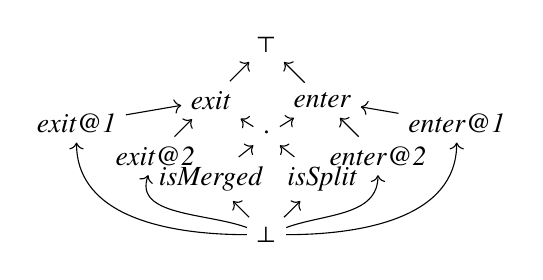
\begin{tikzpicture}
      \node (top) {$\top$} ;

      \node[below left of=top] (exit) {$\mathit{exit}$} ;
      \node[below right of=top] (enter) {$\mathit{enter}$} ;

      \path[->]
      (exit) edge (top)
      (enter) edge (top) ;

      \node[below of=exit] (merge) {$\mathit{isMerged}$} ; 
      \node[below of=enter] (split) {$\mathit{isSplit}$} ;

      \node[left of=merge] (1) {} ;
      \node[above left of=1] (exit1) {$\mathit{exit@1}$} ;
      \node[below left of=exit] (exit2) {$\mathit{exit@2}$} ;

      \path[->]
      (exit1) edge (exit)
      (exit2) edge (exit)
      ;

      \node[right of=split] (2) {} ;
      \node[above right of=2] (enter1) {$\mathit{enter@1}$} ;
      \node[below right of=enter] (enter2) {$\mathit{enter@2}$} ;

      \path[->]
      (enter1) edge (enter)
      (enter2) edge (enter)
      ;

      \node[below right of=merge] (bottom) {$\bot$} ;

      \node (state) at ($(top)!0.475!(bottom)$) {$\cdot$} ;
      
      \path[->]
      (merge) edge (state)
      (split) edge (state)
      (state) edge (exit)
      (state) edge (enter)
      ;
      
      \path[->]
      (bottom) edge[out=180, in=-90] (exit1)
      (bottom) edge[out=160, in=-110] (exit2)
      (bottom) edge[out=0, in=-90] (enter1)
      (bottom) edge[out=20, in=-90] (enter2)
      (bottom) edge (merge)
      (bottom) edge (split)
      ;
      
    \end{tikzpicture}

  }
  \caption{Modular Room motif and the corresponding action lattice}
  \label{fig:ModularRoom}
\end{figure}

\begin{example}[Modular Room motif\cref{ft:detailed}]
  \label{ex:ModularRoom}
  \Cref{fig:MR:motif} shows the map and the external interface of the Modular Room motif.  
  The map has two nodes representing rooms composing the modular room and one node representing a logical component that keeps track of the state of the modular room (split or merged).  The node interface at the latter node (not shown) has two actions, $\actionname{isMerged}$ and $\actionname{isSplit}$, used to signal the state of the modular room.  The node interfaces at the two former nodes (not shown) are the same as the external interface of the motif.  The association of the $\actionname{exit}$ and $\actionname{enter}$ actions at these nodes with the corresponding external actions are established through the action lattice (\cref{fig:MR:lattice}) and the interaction constraint.  For example, the interaction constraint can be written as a conjunction of ``local'' constraints, \eg

  \noindent
  \parbox[b]{0.9\columnwidth}{%
    $\begin{aligned}
      \dots &\land \Big(\actionname{isMerged} \land \exists n \bigl(\predicatename{Room}(n)\bigr): \actionat{n}{\actionname{exit}} \implies \forall n \bigl(\predicatename{Room}(n)\bigr), \actionat{n}{\actionname{exit}}\Big)\\
      &\land \Big(\actionname{isSplit} \land \exists n \bigl(\predicatename{Room}(n)\bigr): \actionat{n}{\actionname{exit}} \implies \exists! n \bigl(\predicatename{Room}(n)): \actionat{n}{\actionname{exit}}\bigr)\Big)
      \land \dots {}
    \end{aligned}$

  }
  %
  \qed
\end{example}

We model structured CPSs as trees with motifs at all internal nodes and atomic components defining the system behaviour at the leaves. The children of each internal node correspond to the nodes of the map of the motif.  See~\cite{BCK26-Motifs} for a detailed example.

As usual, the operational semantics of such assemblies is given in terms of \glspl{lts} materialised by the same kind of objects for both atomic components and composed systems, allowing hierarchical composition.  Below, we reproduce the definition of object from~\cite{BCK26-Motifs}. 
%
Operational semantics is straightforward: measures, knob values and disturbances are plugged in as input-output pairs and transformed within motifs by aggregations and profiles; component actions are synchronised within each motif in accordance with the interaction constraint.  Sets of actions that satisfy the interaction constraint\mdash and can therefore be synchronised\mdash are called \emph{interactions}.\footnote{%
%
Every interaction consists of one external action and a set of corresponding internal ones. 
%
} Formal definition presented in~\cite{BCK26-Motifs} is limited to \emph{closed instantiations}, where an object is plugged into every node of a motif.  However, a straightforward conservative extension allows one to define the semantics in the general case, including \emph{open instantiations}, where some nodes do not have objects plugged in.

\begin{definition}[Object]
  \label{defn:object}
  An \emph{object} $\object$ implementing the interface $\tuple{\actions,
    \vectorspace_{\measurerange}, \vectorspace_{\knobrange}, \vectorspace_{\disturbancerange}, \measurerange, \knobrange, \disturbancerange}$ is an entity that can be given an operational semantics in the form of \pgls{lts} $\semantics{\object} = \tuple{2^{\actions} \times \measurerange \times \knobrange, \actions \times \knobrange \times \disturbancerange, {\goesto{}}}$, 
  such that
  \begin{itemize}
    \item for any $
        (
        \enabled{\actions}
        , \measure
        , \knob
        ) 
        \goesto{\action, \widetilde{\knob}, \disturbance} 
        (
        \enabled{\actions}'
        , \measure'
        , \knob'
        )
        $, 
    we have 
    $\action \in \enabled{\actions}$ and 
    $\knob' = \widetilde{\knob}$,
    
    \item for any               % state
    $\tuple{\enabled{\actions}
    , \measure
    , \knob
    }$,
    $\knob' \in \knobrange$, and
    $\disturbance \in \disturbancerange$,
    there exists
    %% $\enabled{\actions}'$
    %% , $\measure'$
    %% , such that
    $
        (
        \enabled{\actions}
        , \measure
        , \knob
        )
        \goesto{\bot, \knob', \disturbance}
        (
        \enabled{\actions}'
        , \measure'
        , \knob'
        )
        $.
  \end{itemize}
\end{definition}

The state of an object is thus defined by the set of \emph{enabled actions} and the current measurements and knob positions.  The conditions imposed on the transition relation mean that
%
\begin{textlist}
\item only enabled actions can be fired%
  ,
  
\item the knob positions can only be set externally and are not affected by the behaviour of the object%
  , and 
  
\item the bottom action is always enabled%
  .
\end{textlist}

The precise definition of the operational semantics of objects is intentionally left open to be able to accommodate objects of different natures: standard discrete automata, timed automata, hybrid automata, \etc

\subsection{Control Motifs}
\label{secn:control-motifs}

Based on Fig.~\ref{fig:CL}, we consider the basic control signals: measures $\measure$, reference values for these measures $\setpoint{\measure}$, and knobs $\knob$, a tunable signal that allows leveraging the measure signal. In addition, one may consider an external disturbance $\disturbance$. 

Consider an object that implements the interface $\tuple{\actions, 
  \vectorspace_{\measurerange}, \vectorspace_{\knobrange}, \vectorspace_{\disturbancerange}, \measurerange, \knobrange, \disturbancerange}$.  Its control is realized by a \emph{control function} 
  $\control: 2^{\actions} \times \vectorspace_{\measurerange} \times \vectorspace_{\knobrange} \times \vectorspace_{\measurerange} \times \vectorspace_{\disturbancerange} \rightarrow \vectorspace_{\knobrange}$.
Given the current set of enabled actions $\enabled{\actions} \subseteq \actions$ and the current measure $\measure \in \measurerange$, the knob position $\knob \in \knobrange$, a reference value $\setpoint{\measure} \in \measurerange$, and , the disturbance $\disturbance \in \disturbancerange$, the control function defines the new value of the knob $\knob' = \control(\enabled{\actions}, \measure, \knob, \setpoint{\measure}, \disturbance) \in \knobrange$ of the object.

We define \emph{control motifs}, which are a special case of motifs in \cref{defn:motif:1,defn:motif:2} characterised by such control functions.  We put $\motif_{\control} = \tuple{
  \{\singleton\}
  ,\internal{\interface}
  ,\external{\interface}
  ,\identity_{\aggregation}
  ,\control
  ,\identity_{\distprofile}
  ,\constraint[1:1]
}$, where
%
\begin{textlist}
 \item
   $\listset{\singleton}$ is a singleton map (one node, no edges, no predicates)%
   ,
 \item
   $\internal{\interface}_{\control} = \tuple{\actions,
   \vectorspace_{\measurerange}, \vectorspace_{\knobrange}, \vectorspace_{\disturbancerange}, \measurerange, \knobrange, \disturbancerange}$%
   ,
 \item
   $\external{\interface}_{\control} = \tuple{\actions,
   \vectorspace_{\measurerange}, \vectorspace_{\measurerange}, \vectorspace_{\disturbancerange}, \measurerange, \measurerange, \disturbancerange}$%
   ,
 \item 
   $\identity_{\aggregation}: 2^{\actions} \times \vectorspace_{\measurerange} \rightarrow \vectorspace_{\measurerange}$ and
   $\identity_{\distprofile}: 2^{\actions} \times \vectorspace_{\measurerange} \times \vectorspace_{\disturbancerange} \rightarrow \vectorspace_{\disturbancerange}$ are projections on the corresponding last components of their arguments%
   ,
 \item
   the control function $\control$ plays the role of the profile%
   , and
 \item
   $\constraint[1:1] = \bigwedge_{\action \in \actions} (\actionat{\external{}}{\action} \Leftrightarrow \actionat{\singleton}{\action})$%
   .
\end{textlist}

In the external interface of a control motif, the knob is replaced by the reference values of the measures.
We do not impose any constraints on the nature of the control function. However, in this paper, we do limit ourselves to \emph{linear} controllers.

\section{Control of Structured Motifs}
\label{secn:backgr-control}
In this section, the definition of motifs and the linear control formulation are linked. Then, the focus is made on hierarchical systems, specifying the plant formulation for motifs whose map is a tree. We illustrate these elements with the example of smart building detailed in~\cite{BCK26-Motifs}.

Beforehand, we introduce {\em transfer functions}, which are the necessary background on the control theory formulation. 
Indeed, both the plant $\plant$ and the controller $\controller$ are represented using transfer functions. A transfer function represents the transformation of signals, \eg how the knob signal $\knob$ affects the measure signal $\measure$. Thus, this can be written as
\(
\measure = \plant \knob,
\)
where a simple linear relation describes the system behaviour. 
The notions of plant, controller, and their transfer function can now be linked to the motifs defined in \cref{secn:struct}.

\subsection{Linking Control Formulation \& Motifs}
\label{secn:control-problem}

Let us first consider a motif $\motif$ in the most general case. 
The \emph{plant} transfer function $\plant$ captures the impact of the changes of knobs $\knob$ on measures $\measure$. This mathematical model links elements in motif's external interface $\external{\interface}$, with $\knob \in \external{\knobrange}$ and $\measure \in \external{\measurerange}$.
The impact of disturbances $\disturbance$ on measurements is also taken into account in the model, \eg by artificially increasing the measurement vector $\measure$ with disturbances. 

The plant $\plant$ is thus a partial view of a motif, only concerned with the evolution of the external interface signals. Its dependence on internal elements can be explored in the case where the map is specified, as presented in the next subsection.

We now consider a \emph{control motif} $\motif_{\control}$. 
The \emph{controller} $\controller$ captures the impact of the references and the measures (often through their difference, \ie the reference tracking error) and the disturbances $\disturbance$ on the knobs signal:
$
\knob = \controller (\setpoint{\measure},\measure, \disturbance).
$
Thus, the controller $\controller$ models the link between the elements of the internal and external interfaces of the control motif $\motif_{\control}$. 

\begin{example}{(Room temperature control in a Smart Building)}
\label{ex:control-formulation}
The room \textbf{plant} \(\plant_{\predicatename{Room}}\) models the impact of the knob (here the heating power $\knob_{\predicatename{Room}}=\power_{\predicatename{Room}}$) on the measure (here the room temperature $\measure_{\predicatename{Room}} = \temperature_{\predicatename{Room}}$), under disturbances $\disturbance_{\predicatename{Room}}$ (neighboring temperatures, radiations, etc.). 
%
We define $x$ as the set of all relevant measures and disturbances:
$
    x \bydef \left(\begin{array}{c} \measure_{\predicatename{Room}} \\ \disturbance_{\predicatename{Room}} \end{array}\right).
$
The indoor temperatures evolution is modeled as:
\begin{equation}
\label{eq:room-ss-model}
\left\{
    \begin{array}{l}
        x' = A x + B \knob_{\predicatename{Room}}, \\
        \measure_{\predicatename{Room}} = C x
    \end{array}
\right.
\end{equation}
where $x'$ denotes either the derivative of $x$ in the continuous-time case, or its value at the next time-step in the discrete-time case. 
$A$ and $B$ are matrices taking into account the convection, thermal resistances, and capacity of the various elements around the room. The matrix $C$ selects the room temperature among the disturbances.

The transfer function \(\plant_{\predicatename{Room}}\) is then computed using the model matrices:
$
\plant_{\predicatename{Room}}(s) = C (s I -A) ^{-1} B
$,
with $I$ the identity matrix of adequate size and $s$ the complex variable. 

The room \textbf{controller} \( \controller_{\predicatename{Room}}\) computes the heat power knob value \(\knob_{\predicatename{Room}}\) based on the target temperature \(\setpoint{\measure}_{\predicatename{Room}}\), the room measured temperature \(\measure_{\predicatename{Room}}\) and all the disturbances. 
For the linear time-invariant system that we consider, the optimal controller can be computed as a state feedback, with precompensation for the reference tracking:
\begin{equation}
    \label{eq:ex:control:optimal}
    \controller_{\predicatename{Room}} (\setpoint{\measure}_{\predicatename{Room}},\measure_{\predicatename{Room}}, \disturbance_{\predicatename{Room}}) = -\controlgain \left(\begin{array}{c} \measure_{\predicatename{Room}} \\ \disturbance_{\predicatename{Room}} \end{array}\right) + \precomp \setpoint{\measure}_{\predicatename{Room}},
\end{equation}
where \( \controlgain \) is the state feedback gain; and \( \precomp \) is the precompensation gain, both being vectors of appropriate sizes. The computation of the controller gains is detailed in \cite{BCK26-Motifs}.
  %
  \qed
\end{example}

\subsection{Hierarchical Control}

We consider CPSs with a hierarchical structure, in which there is at least one controller. At a given level, the motif map and interfaces are instantiated, and we fix an order on the nodes of the map.
Note that here the disturbances are not explicitly written in the following formulations to simplify, as they can be considered as part of the measurement vector $\measure$ extended with disturbances.

The plant $\plant$ modeling the knobs-to-measures behaviour of the motif $\motif$, can be expressed using the profile function $\profile$, the aggregation function $\aggregation$, and recursively over the lower level motifs. 
At a given level, the measure \(\measure \in \external{\measurerange}\) is the \emph{aggregation} of the measures \(\measure_i\) of the lower levels:
\(
\measure = \aggregation \measurevect,
\)
with \( \measurevect = (\measure_1, \cdots, \measure_i, \cdots, \measure_n)^T \in \internal{\measurerange}\) (internal interfaces).

The controller \(\controller\) computes the knob \(\knob \in \external{\knobrange}\) (external interfaces), that is distributed among the lower levels as \(\knob_i\) by the \emph{profile} function \(\profile\):
\(
\label{eq:profile}
    \knobvect = \profile \knob,
\)
with \( \knobvect = (\knob_1, \cdots, \knob_i, \cdots, \knob_n)^T \in \internal{\knobrange}\) (internal interfaces).
%
The measure at a lower level can be derived from the value of the knob that was enforced, and is modelled by \(\subplant_i\), the \emph{subsystem} transfer function
\(
    \measure_i = \subplant_i \knob_i
\).

The hierarchical control consists then in designing \( \controller \) to regulate the \emph{plant} \(\plant\), recursively formulated as
$
\plant = \aggregation \mathbf{\subplant} \profile,
$
with \(\mathbf{\subplant} \bydef (\subplant_1, \cdots, \subplant_i, \cdots, \subplant_n) \times \textbf{I}_n\).

\begin{example}
Following Example \ref{ex:control-formulation}, 
consider a floor composed of $n$ rooms. 
The floor model \( \plant_\predicatename{Floor}\) based on the room models \( \plant_{\predicatename{Room},i} \) and the floor aggregation and profile matrices. 
At the lower level, each room is controlled by a feedback controller, their equivalent closed-loop transfer function is thus:
\[ \subplant_{\predicatename{Room},i} = \dfrac{\controller_{\predicatename{Room},i} \plant_{\predicatename{Room},i} }{1 + \controller_{\predicatename{Room},i} \plant_{\predicatename{Room},i}}\,. \] 
%
The floor power is computed as the sum of all the power used in the rooms.
The aggregation $\aggregation_\predicatename{Floor}$ is then:
$
\aggregation_\predicatename{Floor} =     
\bigl(\begin{array}{ccc} 1 & \cdots & 1 \end{array}\bigr)^T .
$

\noindent The profile $\profile_\predicatename{Floor}$ distributes the temperature references between the rooms: 
$
\profile_\predicatename{Floor} = \bigl(\begin{array}{ccc} \alpha_1 & \cdots & \alpha_n \end{array}\bigr),
$
where $\alpha_i$ is a scaling factor depending on the room usage.  It is equal to $1$ if the room is occupied, $0.8$ if the room is empty or a hallway, and $0.7$ in the server room.
%
Overall, the floor plant is then
$
\plant_\predicatename{Floor} = \aggregation_\predicatename{Floor} \mathbf{\subplant_{\predicatename{Room}}} \profile_\predicatename{Floor},  
$
with \( \mathbf{\subplant_{\predicatename{Room}}} = \left( \subplant_{\predicatename{Room},1} ~ \cdots ~ \subplant_{\predicatename{Room},n} \right)  \times \textbf{I}_n \).
%
\qed
\end{example}

\section{Motif Refinement}
\label{secn:def-refinement}
\label{secn:refinement}
This section aims to address \ref{rq:refinement}.  Based on the motif model, we introduce a control-compatible notion of a motif refinement and state its basic properties.
%
More precisely, we propose two kinds of motif refinement:
\begin{textlist}
\item refinement of interfaces, potentially introducing new nodes, and
\item refinement of the map by replicating existing nodes.
\end{textlist}
These can be combined arbitrarily to obtain more complex motif refinements.

\subsection{Motif Refinement Definitions}
\label{secn:refinement:defs}

\paragraph{Refinement of interfaces}
This kind of refinement follows the classical schema for interface and contract refinement: covariant expansion on the inputs and contravariant expansion on the outputs.  Although every control-related element of an interface is viewed as an input or an output of a motif, these roles change depending on whether the corresponding interface is internal or external (see \cref{note:io}).  Furthermore, the particularity of the proposed refinement notions is that we allow expanding the dimensions of the corresponding vector spaces.  For example, the refining motif can provide entirely new measures not present in the refined one so long as the range of values does not grow for the existing measures.  The ensuing necessity to simultaneously address the dual (co- and contravariant) expansion and the projection of the underlying vector spaces leads us to define separate notions of refinement for internal and for external interfaces.

\begin{definition}[Map containment]
  \label{defn:map:contain}
  A map $\map_{1}$ is \emph{contained} in another map $\map_{2}$, denoted $\map_{1} \subseteq \map_{2}$, if
  \begin{textlist}
  \item $\nodes_{1} \subseteq \nodes_{2}$,
  \item $\edges_{1} = \edges_{2} \cap \nodes_{1}^2$, \ie there are no ``new'' edges between the ``old'' nodes,
  \item $\predicates_{1} \subseteq \predicates_{2}$, and
  \item for any $P \in \predicates_{1}$, we have $\map_{1}.P = \project[x]{\map_{2}.P}{\nodes_{1} \cup \edges_{1}}$, \ie the meaning of the predicates does not change.
  \end{textlist}
\end{definition}

\begin{definition}[Interface refinement]
  \label{defn:refine:interface}
  Let $\interface_{i} = \tuple{
    \actions_{i}
    , 
    \vectorspace_{\measurerange,i}
    ,
    \vectorspace_{\knobrange,i}
    ,
    \vectorspace_{\disturbancerange,i}
    ,
    \measurerange_i
    ,
    \knobrange_i
    ,
    \disturbancerange_i
  }$ (with $i=1,2$) be two interfaces, such that 
%
  \begin{textlist}
  \item $\actions_{1} \subseteq \actions_{2}$ and
  \item $\vectorspace_{\measurerange,1}$, $\vectorspace_{\knobrange,1}$, and $\vectorspace_{\disturbancerange,1}$ are sub-spaces of $\vectorspace_{\measurerange,2}$, $\vectorspace_{\knobrange,2}$, and $\vectorspace_{\disturbancerange,2}$, \resp[]
  \end{textlist}
%
  Denote $\project[force:target]{}{\vectorspace_{*,1}}: \vectorspace_{*,2} \rightarrow \vectorspace_{*,1}$, for $* \in \listset{\measurerange, \knobrange, \disturbancerange}$, the corresponding vector space projections.  Whenever unambiguously determined by the context, we will write 
  $\project{}{\vectorspace_{*,1}}$ 
  without the index indicating the target space.


  Interface $\interface_1$ is \emph{externally refined} by $\interface_2$, denoted $\interface_1 \external{\isrefinedby} \interface_2$, if
%
  $
  \project{\measurerange_2}{\vectorspace_{\measurerange,1}} \subseteq \measurerange_1
  \text{, }
  \knobrange_1 \subseteq \project{\knobrange_2}{\vectorspace_{\knobrange,1}}
  \text{, and }
  \disturbancerange_1 \subseteq \project{\disturbancerange_2}{\vectorspace_{\disturbancerange,1}}
  $.
%
  It is refined \emph{internally}, denoted $\interface_1 \internal{\isrefinedby} \interface_2$, if
%
  $
  \measurerange_1 \subseteq \project{\measurerange_2}{\vectorspace_{\measurerange,1}} 
  \text{, }
  \project{\knobrange_2}{\vectorspace_{\knobrange,1}} \subseteq \knobrange_1
  \text{, and }
  \project{\disturbancerange_2}{\vectorspace_{\disturbancerange,1}} \subseteq \disturbancerange_1
  $.
\end{definition}

Denote $\lift[force:target]{}{\vectorspace_{*,2}}$ (for $* \in \listset{\measurerange, \knobrange, \disturbancerange}$) the lifting corresponding to the projection $\project[force:target]{}{\vectorspace_{*,1}}$, that is, for $X \subseteq \vectorspace_{*,1}$, we have $\lift[force:target]{X}{\vectorspace_{*,2}} \bydef \bsetdef{x \in \vectorspace_{*,2}}{\project[force:target]{x}{\vectorspace_{*,1}} \in X}$.  As for projection, we will omit the exponent whenever unambiguously determined by the context.

\begin{definition}[Refinement of motif interfaces]
  \label{defn:interface:refinement}
  Let $\motif_{i} = \btuple{
%
    \map_{i}
%
    ,(\interface[n]_{i})_{n \in \map}
%
    ,\external{\interface}_i
%
    ,\aggregation_i
%
    ,\profile_i
%
    ,\distprofile_i
%
    ,\constraint_i
%
  }$ (with $i = 1,2$) be two motifs.
  Motif $\motif_{1}$ is \emph{interface-refined} by $\motif_{2}$, denoted $\motif_{1} \isrefinedby[i] \motif_{2}$, if hold
  \begin{textlist}
  \item $\map_{1} \subseteq \map_{2}$,
  \item $\external{\interface}_1 \external{\isrefinedby} \external{\interface}_2$,
  \item for every node $n \in \map$, $\interface[n]_1 \internal{\isrefinedby} \interface[n]_2$,
  \item $\constraint_{1} \Rightarrow \exists_{\actions[\motif_{2}]\setminus \actions[\motif_{1}]} \constraint_{2}$, \ie for any interaction $\interaction_{1} \subseteq \actions[\motif_{1}]$ allowed in $\motif_{1}$, there exists an interaction $\interaction_{2} \subseteq \actions[\motif_{2}]$ allowed in $\motif_{2}$, such that $\interaction_{1} \subseteq \interaction_{2}$ and $\interaction_{2}\setminus\interaction_{1} \subseteq \actions[\motif_{2}]\setminus \actions[\motif_{1}]$
    and
  \item all three of the aggregation, control and disturbance profiles commute with the corresponding projections, \ie
  \end{textlist}
%
  \begin{itemize}

  \item
    $\aggregation_{1}\bigl(\enabled{\actions} \cap \internal{\actions}_{1}, \project{\measure}{\internal{\vectorspace}_{\measurerange,1}}\bigr) = \project{\aggregation_{2}(\enabled{\actions}, \measure)}{\external{\vectorspace}_{\measurerange,1}}$,
    %
    for all $\enabled{\actions} \subseteq \internal{\actions}_{2}$ and $\measure \in \lift{\internal{\measurerange}_{1}}{\internal{\vectorspace}_{\measurerange,2}}$,
    
  \item
    $\profile_{1}\bigl(\enabled{\actions} \cap \internal{\actions}_{1}, \project{\measure}{\internal{\vectorspace}_{\measurerange,1}}, \project{\knob}{\internal{\vectorspace}_{\knobrange,1}}, \project{\knob'}{\external{\vectorspace}_{\knobrange,1}}, \project{\disturbance}{\external{\vectorspace}_{\disturbancerange,1}}\bigr) =
    \project{\profile_{2}\bigl(\enabled{\actions}, \knob, \knob', \disturbance\bigr)}{\internal{\vectorspace}_{\knobrange, 1}},$
    %
    for all $\enabled{\actions} \subseteq \internal{\actions}_{2}$, $\measure \in \lift{\internal{\measurerange}_{1}}{\internal{\vectorspace}_{\measurerange,2}}$, $\knob \in \internal{\knobrange}_{2}$, $\knob' \in \lift{\external{\knobrange}_{1}}{\external{\vectorspace}_{\knobrange, 2}}$ and $\disturbance \in \lift{\external{\disturbancerange}_{1}}{\external{\vectorspace}_{\disturbancerange, 2}}$, 
    
  \item
    $\distprofile_{1}\bigl(\enabled{\actions} \cap \internal{\actions}_{1}, \project{\measure}{\internal{\vectorspace}_{\measurerange,1}}, \project{\disturbance}{\external{\vectorspace}_{\disturbancerange,1}}\bigr) = \project{\distprofile_{2}(\enabled{\actions}, \measure, \disturbance)}{\internal{\vectorspace}_{\disturbancerange, 1}}$,
    %
    for all $\enabled{\actions} \subseteq \internal{\actions}_{2}$, $\measure \in \lift{\internal{\measurerange}_{1}}{\internal{\vectorspace}_{\measurerange,2}}$, and $\disturbance \in \lift{\external{\disturbancerange}_{1}}{\external{\vectorspace}_{\disturbancerange, 2}}$.
    
  \end{itemize}
  
\end{definition}

Notice that the refinement notion in \defn{interface:refinement} allows new nodes to be added to the refining motif.  The internal interface associated with the new nodes would contribute new dimensions to the internal interface of the refining motif. However, according to \defn{refine:interface} we still have $\internal{\interface}_1 \internal{\isrefinedby} \internal{\interface}_2$ (with $\internal{\interface}_1$, $\internal{\interface}_2$ as in \defn{motif:1}).

\begin{example}
  \label{ex:refinement:motif}
  Straightforward examples of refinement of motif interfaces are
  \begin{textlist}
  \item refining a motif by introducing new nodes without modifying the existing ones, 
  \item adding new measures, knobs or disturbances to existing nodes, and
  \item improving the ``quality'' of the aggregation, or control or disturbance profiles.
  \end{textlist}
  %
  \qed
\end{example}

\paragraph{Node replication}
A map $\map_2$ refines another map $\map_1$ if $\map_1$ can be obtained from $\map_2$ by contracting some of the edges.  To define this formally, we need the notion of node lifting.  Let $\mu_i = \tuple{\nodes_i, \edges_i}$, for $i = 1,2$.

\begin{definition}[Node lifting]
  \label{defn:lifting}
  Let $r: \nodes_2 \rightarrow \nodes_1$ be a surjective mapping. %% ($\bsetdef{r^{-1}(n)}{n \in \nodes_1}$ is a partition of $\nodes_2$).
  The
  \emph{lifting of a node $n \in \nodes_1$ along $r$} is the sub-graph $\btuple{r^{-1}(n), r^{-1}(n)^2 \cap \edges_2}$ of $\mu_2$.
\end{definition}

\begin{definition}[Map refinement]
  \label{defn:refine:map}
  A map $\map_1$ is refined by $\map_2$, denoted $\map_1 \isrefinedby \map_2$, if there exists a surjective mapping $r : \nodes_2 \rightarrow \nodes_1$, such that 
%
  \begin{textlist}
  \item
    the lifting of each node $n \in \nodes_1$ along $r$ is a connected graph%
    , 
  \item
    two nodes in $\nodes_1$ are connected iff so are their liftings
    along $r$, \ie
    $\edges_1 = \bsetdef{(n_1, n_1')}{\exists n_2 \in r^{-1}(n_1), n_2' \in r^{-1}(n_1'): (n_2, n_2') \in \edges_2}$%
    ,
  \item $\predicates_{1} \subseteq \predicates_{2}$%
    ,
  \item the lifting of a node satisfies the same predicates as the lifted node, \ie[,] for all $n \in \nodes_{2}$ and $P \in \predicates_{1}$, holds $P(n) = P\bigl(r(n)\bigr)$%
    ,
    and
  \item similarly for the edges, \ie[,] for all $(n, n') \in \edges_{2}$ and $P \in \predicates_{1}$, either $r(n) = r(n')$ or $P(n,n') = P\bigl(r(n), r(n')\bigr)$%
    .
  \end{textlist}

  We call $r$ the \emph{witness mapping} of the refinement.
\end{definition}

For the remainder of this section, let us fix two motifs $\motif_{i} = \btuple{
%
    \map_{i}
%
    ,(\interface[n]_{i})_{n \in \map_{i}}
%
    ,\external{\interface}
%
    ,\aggregation_{i}
%
    ,\profile_{i}
%
    ,\distprofile_{i}
%
    ,\constraint_{i}
%
}$ (with $i = 1,2$) with the same external profile, and such that $\map_{1} \isrefinedby \map_{2}$ with a witness mapping $r: \nodes_{2} \rightarrow \nodes_{1}$.
Assume that, for every $n_1 \in \nodes_{1}$ and every $n_2 \in r^{-1}(n_1)$, we have $\interface[n_2]_{2} = \interface[n_1]_{1}$. (Hence, for $n \in \map_{1}$, we can skip the index on the interface $\interface[n]$ and its components.)
As for \defn{interface:refinement}, it follows immediately from \defn{refine:interface} that $\internal{\interface}_1 \internal{\isrefinedby} \internal{\interface}_2$.

Aggregation $\aggregation_2$ refines $\aggregation_1$ if the measures in $\internal{\interface}_2$ can be ``pre-aggregated'' %% before the application of $\aggregation_1$
so that the aggregated measures coincide with those obtained by $\aggregation_2$.

\begin{definition}[Aggregation refinement]
  \label{defn:refine:aggreg}
  An aggregation $\aggregation_1$ is refined by $\aggregation_2$, denoted $\aggregation_1 \isrefinedby \aggregation_2$, if there exists a family of \emph{pre-aggregation} mappings $f = (f_n)_{n \in \map_1}$ with $f_n: \bigl(\vectorspace[n]_{\measurerange}\bigr)^{|r^{-1}(n)|} \rightarrow \vectorspace[n]_{\measurerange}$, such that $\aggregation_2 = \aggregation_1 \circ (f, \project{}{\external{\vectorspace}_{\disturbancerange,1}})$, \ie
  \[
  \aggregation_2(
  \enabled{\actions},
  \measure,
  \disturbance
  )
  =
  \aggregation_1\bigl(
  \enabled{\actions} \cap \internal{\actions}_{1},
  f(\measure),
  \project{\disturbance}{\external{\vectorspace}_{\disturbancerange,1}}
  \bigr)
  \,,
  \]
  for all $\enabled{\actions} \subseteq \internal{\actions}_{2}$, $\measure \in \internal{\vectorspace}_{\measurerange,2}$ and $\disturbance \in \external{\vectorspace}_{\disturbancerange,2}$.
\end{definition}

Control profile refinement is defined similarly to the aggregation one. Recall that, in addition to the set of enabled actions, a profile takes four parameters to compute the updated positions of the internal knobs: the current internal values of the measures, the current positions of the internal knobs, the position of the external knob, and the external disturbance.  Thus, profile $\profile_2$ refines $\profile_1$ if, similarly to \defn{refine:aggreg}, the current internal values of the measures and the current positions of the internal knobs can be ``pre-aggregated'' before the application of $\profile_1$.  Conversely, for each node $n \in \map_1$, the result of this application must be further redistributed to the nodes in $r^{-1}(n)$.

\begin{definition}[Control profile refinement]
  \label{defn:refine:profile}
  Control profile $\profile_1$ is refined by $\profile_2$, denoted $\profile_1 \isrefinedby \profile_2$, if there exist three families of mappings:
%
  \begin{itemize}

  \item measure pre-aggregation $f = (f_n)_{n \in \map_1}$ %% with
    as in \defn{refine:aggreg},%

  \item knob pre-aggregation $g = (g_n)_{n \in \map_1}$ with
    $
    g_n: \bigl(\vectorspace[n]_{\knobrange}\bigr)^{|r^{-1}(n)|} \rightarrow \vectorspace[n]_{\knobrange}
    $,%

  \item knob re-distribution $h = (h_n)_{n \in \map_1}$ with
    $
    h_n: \bigl(\vectorspace[n]_{\measurerange}\bigr)^{|r^{-1}(n)|} \times  \bigl(\vectorspace[n]_{\knobrange}\bigr)^{|r^{-1}(n)|} \times \vectorspace[n]_{\knobrange} \rightarrow \bigl(\vectorspace[n]_{\knobrange}\bigr)^{|r^{-1}(n)|}
    $,%
    
  \end{itemize}
%
  such that $g_n \circ h_n = \project{}{3}$, \ie[], for all $n \in \map_{\motif_1}$, $y \in \prod_{n' \in r^{-1}(n)}\vectorspace[n']_{\measurerange,2}$, $u \in \prod_{n' \in r^{-1}(n)} \vectorspace[n']_{\knobrange,2}$ and $u_n \in \vectorspace[n]_{\knobrange,1}$, we have
  $g_n\bigl(h_n (y,u,u_n)\bigr) = u_n$
  and also $\profile_2 = h \circ \profile_1 \circ (f, g, \project{}{\external{\vectorspace}_{\knobrange,1}}, \project{}{\external{\vectorspace}_{\disturbancerange,1}})$, \ie
    \begin{equation}
    \label{eq:profile-reft}
      \profile_2(
      \enabled{\actions},
      \measure,
      \knob,
      \external{\knob},
      \disturbance
      )
      =
      h\Big(
      \measure,
      \knob,
      \profile_1\bigl(
      \enabled{\actions} \cap \internal{\actions}_{1},
      f(\measure),
      g(\knob),
      \project{\external{\knob}}{\external{\vectorspace}_{\knobrange_1}},
      \project{\disturbance}{\external{\vectorspace}_{\disturbancerange,1}}
      \bigr)
      \Big)
      \,,
    \end{equation}
    for all $\enabled{\actions} \subseteq \internal{\actions}_{2}$, $\measure \in \internal{\vectorspace}_{\measurerange,2}$, $\knob \in \internal{\vectorspace}_{\knobrange,2}$, $\external{\knob} \in \external{\vectorspace}_{\knobrange,2}$ and $\disturbance \in \external{\vectorspace}_{\disturbancerange,2}$.
\end{definition}

Disturbance profile refinement is defined similarly to that of the control profile.

\begin{definition}[Disturbance profile refinement]
  \label{defn:refine:distprofile}
  Disturbance profile $\distprofile_1$ is refined by $\distprofile_2$, denoted $\distprofile_1 \isrefinedby \distprofile_2$, if there exist two families of mappings:
%
  \begin{itemize}

  \item measure pre-aggregation $f = (f_n)_{n \in \map_1}$ as in \defn{refine:aggreg},%

  \item disturbance re-distribution $t = (t_n)_{n \in \map_1}$ with
    $
    t_n: \bigl(\vectorspace[n]_{\measurerange}\bigr)^{|r^{-1}(n)|} \times \vectorspace[n]_{\disturbancerange} \rightarrow \bigl(\vectorspace[n]_{\disturbancerange}\bigr)^{|r^{-1}(n)|}
    $,%
    
  \end{itemize}
%
  such that $\distprofile_2 = t \circ \distprofile_1 \circ (f, \project{}{\external{\vectorspace}_{\disturbancerange,1}})$, \ie
  $\distprofile_2(
      \enabled{\actions},
      \measure,
      \disturbance
      )
      =
      t\Big(
      \measure,
      \distprofile_1\bigl(
      \enabled{\actions} \cap \internal{\actions}_{1},
      f(\measure),
      \project{\disturbance}{\external{\vectorspace}_{\disturbancerange,1}}
      \bigr)
      \Big)$,
    for all $\enabled{\actions} \subseteq \internal{\actions}_{2}$, $\measure \in \internal{\vectorspace}_{\measurerange,2}$ and $\disturbance \in \external{\vectorspace}_{\disturbancerange,2}$.
\end{definition}

To define the inteaction constraint refinement, we have to explain how individual actions of every interface $\interface[n]_1$ are realised in terms of actions of the interfaces $(\interface[n']_2)_{n' \in r^{-1}(n)}$.

\begin{definition}[Interaction constraint refinement]
  \label{defn:refine:constraint}
  Interaction constraint $\constraint_1$ is refined by $\constraint_2$, denoted $\constraint_1 \isrefinedby \constraint_2$ if, there exists a family of constraints $\bigl(\constraint_{\action})_{\action \in \internal{\interface}_{1}}$, such that 
    \begin{textlist}
    \item
      each constraint $\constraint_{\action}$ (for $\action \in \actions[n]$) refers precisely to the actions $\actionat{n'}{\action}$ with $n' \in r^{-1}(n)$, and
    \item $\constraint_2 = \constraint_1 \land \bigwedge_{n \in \map_{1}} \bigwedge_{\action \in \actions[n]} (\actionat{n}{\action} \Leftrightarrow \constraint_{\action})$.
    \end{textlist}
\end{definition}

\begin{definition}[Refinement of motif maps]
  \label{defn:refine:motif}
  Let $\motif_1$ and $\motif_2$ be two motifs with $\external{\interface}_1 = \external{\interface}_2$.
  Motif $\motif_1$ is \emph{map-refined} by $\motif_2$, denoted $\motif_1 \isrefinedby[m] \motif_2$, if there exist witness, pre-aggregation and re-distribution mappings $r$, $f$, $g$, $h$, $t$ \resp[], such that 
  \begin{textlist}
  \item $\map_1 \isrefinedby \map_2$, 
  \item for every node $n_1 \in \nodes_{1}$ and every node $n_2 \in r^{-1}(n_1)$, we have $\interface[n_2]_{2} = \interface[n_1]_{1}$,
  \item $\aggregation_1 \isrefinedby \aggregation_2$, $\profile_1 \isrefinedby \profile_2$, $\distprofile_1 \isrefinedby \distprofile_2$ and $\constraint_1 \isrefinedby \constraint_2$.
  \end{textlist}
\end{definition}

\begin{example}
  \label{ex:refinement:map}
  Refinement of motif maps allows replicating existing nodes.  For instance, the Room nodes of the Floor motif (adjacent to the server room in the floor plan in \cref{fig:floor}) could each be replaced by several nodes representing smaller rooms.
  %
  \qed
\end{example}

\subsection{Motif Instantiation}
\label{secn:instantiation}

We now define what it means to instantiate a node of a motif with an object (which could, in turn be a hierarchically composed system).  We generalise the definitions in \cite{BCK26-Motifs} by relaxing the constraints that objects implement precisely the node interfaces and by allowing open instantiations.

\begin{definition}[Instantiation]
  \label{defn:instantiation}
  A \emph{motif instantiation}, denoted $\motif\bigl(\setdef{\object_n/n}{n \in N}\bigr)$, where $\motif$ is a motif, $\nodes \subseteq \map_{\motif}$ is a set of nodes, and, for each node $n \in \nodes$, $\object_n$ an object implementing an interface $\interface$, such that $\interface[n] \external{\isrefinedby} \interface$ of $\motif$.  An instantiation is \emph{closed} if $\nodes$ is the set of all nodes of $\map_{\motif}$.  Otherwise, it is \emph{open}.
\end{definition}

The semantics of $\motif\bigl(\setdef{\object_n/n}{n \in N}\bigr)$ is defined by the following rule, where the changes from the rule in \cite{BCK26-Motifs} are highlighted in red (premises 7 and 8). 
%
\begin{equation}
  \label{eq:motif:sem:general}
  \inferrule{
    \action \in \enabled{\actions}
    \\
    \action = \bigvee_{n \in \map} \action_{n}
    \\
    \knob' \in \external{\knobrange}
    \\
    \bigl(
    \action
    , (\action_{n})_{n \in \map}
    , (\measure_{n})_{n \in \map}
    , \knob
    \bigr) \satisfies \constraint
    \\\\
    (\knob_{n}')_{n \in \map}
    =
    \profile\Tuple{\bigcup_{n \in \map}\enabled[n]{\actions}, (\measure_{n})_{n \in \map}, (\knob_n)_{n \in \map}, \knob'}
    \\
    (\disturbance_{n})_{n \in \map}
    =
    \distprofile\Tuple{\bigcup_{n \in \map}\enabled[n]{\actions}, (\measure_{n})_{n \in \map}, d}
    \\\\
    \textcolor{red}{\forall n \in \nodes},~ \tuple{\enabled[n]{\actions},
      \measure_{n}, \knob_{n}}
    \goesto{\action_n,\, \knob_{n}',\, \disturbance_{n}}
    \tuple{\enabled[n]{\actions}',
      \measure_{n}', \knob_{n}'}
    \\
    \textcolor{red}{\forall n \not\in \nodes,~ \measure_{n}' \in \measurerange_{n}}
    \\\\
    \enabled{\actions}' = \Bsetdef{
      \action' = \bigvee_{n \in \map} \action_n' \in \external{\actions}
    }{
       \action_{n}' \in \enabled[n]{\actions}' 
       \land
       \bigl(
       \action', 
       (\action_{n}')_{n \in \map}
       , (\measure_{n}')_{n \in \map}
       , \knob'
       \bigr) \satisfies \constraint
    }
    \\
    \measure = \aggregation\Tuple{\bigcup_{n \in \map}\enabled[n]{\actions}, (\measure_{n})_{n \in \map}}
    \\
    \measure' = \aggregation\Tuple{\bigcup_{n \in \map}\enabled[n]{\actions}', (\measure_{n}')_{n \in \map}}
  }{
    \tuple{
    \enabled{\actions}
    , \measure
    , \knob
    }
    \goesto{\action,\, \knob',\, \disturbance}
    \tuple{
    \enabled{\actions}'
    , \measure'
    , \knob'
    }
  }
\end{equation}

The generalisation is conservative: the semanitcs of closed instantiations remains the same as in \cite{BCK26-Motifs}.  For open instantiations, the actions associated to the interfaces of non-instantiated nodes are considered to be always enabled; the measures provided can be arbitrary within the corresponding domain.

\begin{proposition}
  \label{prop:semantics:correct}
  $\motif\bigl(\setdef{\object_n/n}{n \in N}\bigr)$ is an object in the sense of \defn{object}.
\end{proposition}

\subsection{Properties of Motif Refinement}
\label{secn:refinement:props}

We provide two basic results about the impact of motif refinement on the behaviour of the coordinated system.  We rely on the following notion of object refinement.  These results correspond to ideal cases, where the input behaviours match exactly and we do not need control-theoretic results to establish the correspondence.  More general results, based on the control-theoretic methodology are presented in \secn{Ctrl-Stability}.

\begin{definition}[Object refinement]
  \label{defn:open:simulation}
  Let $\object_1, \object_2$ be two objects implementing, \resp[,] interfaces $\interface_1, \interface_2$, with $\interface_1 \external\isrefinedby \interface_2$.  We say that $\object_2$ \emph{refines} $\object_1$, denoted $\object_1 \isrefinedby \object_2$, if for any 
  $
  (
  \enabled[1]{\actions}
  , \measure_1
  , \knob_1
  ) 
  \goesto{\action_1, \knob_1', \disturbance_1} 
  (
  \enabled[1]{\actions}'
  , \measure_1'
  , \knob_1'
  )
  $
  in $\semantics{\object_1}$ and any
  $
  (
  \enabled[2]{\actions}
  , \measure_2
  , \knob_2
  )
  $, such that
  $
  \enabled[1]{\actions} = 
  \enabled[2]{\actions} \cap \actions_1
  $,
  $\measure_1 = \project{\measure_2}{\vectorspace{\measurerange_{1}}}$,
  and
  $\knob_1 = \project{\knob_2}{\vectorspace{\knobrange_{1}}}$,
  there exists
  $
  (
  \enabled[2]{\actions}
  , \measure_2
  , \knob_2
  ) 
  \goesto{\action_2, \knob_2', \disturbance_2} 
  (
  \enabled[2]{\actions}'
  , \measure_2'
  , \knob_2'
  )
  $
  in $\semantics{\object_2}$, such that
  $
  \enabled[1]{\actions}' = 
  \enabled[2]{\actions}' \cap \actions_1
  $,
  $\action_1 = \action_2 \cap \actions_1$,
  $\knob_1' = \project{\knob_2'}{\vectorspace{\knobrange_{1}}}$,
  $\disturbance_1 = \project{\disturbance_2}{\vectorspace{\disturbancerange_{1}}}$,
  and
  \[
  \BRsetdef{\project{\measure_2'}{\vectorspace{\measurerange_{1}}}}{
    (
    \enabled[2]{\actions}
    , \measure_2
    , \knob_2
    ) 
    \goesto{\action_2, \knob_2', \disturbance_2} 
    (
    \enabled[2]{\actions}'
    , \measure_2'
    , \knob_2'
    )
  }
  \subseteq
  \BRsetdef{\measure_1'}{
    (
    \enabled[1]{\actions}
    , \measure_1
    , \knob_1
    ) 
    \goesto{\action_1, \knob_1', \disturbance_1} 
    (
    \enabled[1]{\actions}'
    , \measure_1'
    , \knob_1'
    )
  }
  \,.
  \]
\end{definition}

Since object refinement is also a preorder, we formulate the two propositions below for one object plugged into one node of a motif.  By transitivity, both results can be extended to sets of objects implementing the interfaces of several nodes.

The following proposition states that the result of applying an interface-refined motif to essentially the same object refines the initial assembly.  In general, a refined motif cannot be applied to the same object, since the vector spaces in the interface implemented by the object must comprise the corresponding vector spaces in the node interface.  Hence, we refine the object to match the required interface.  Although it is fairly straightforward to construct such an object with minimal necessary adjustments, we opt for a more general, non-constructive result.  Indeed, we claim that any object that refines the initial one while implementing an appropriate interface, achieves the objective.

\begin{proposition}
  \label{prop:simulation}
  Let $\object$ be an object implementing an interface $\interface$, such that $\interface[n]_1 \external{\isrefinedby} \interface$, for some node $n$ of a motif $\motif_1$.  Then $\motif_1 \isrefinedby[i] \motif_2$ implies $\motif_1(\object/n) \issimulatedby \motif_2(\object'/n)$, for any $\object'$ implementing an interface $\interface'$, such that  $\interface[n]_2 \external{\isrefinedby} \interface'$ and $\object \issimulatedby \object'$.
\end{proposition}

For the refinement by node replication, the intuition is that we split the ``work'' among the new nodes.  For example, instead of requiring one radiator to provide a certain amount of heat, we require two radiators to each provide half of that amount.  The difficulty lies in the fact that the control of the nodes is indirect.  For the radiators, \eg[,] we set the power knobs to half the initial value each and expect the produced heat to behave accordingly.  Since the domains of the knobs and of the measures of a motif do not necessarily coincide, it is not possible to make this connection directly in full generality.  However, this can be done for control motifs, which establish a connection between target values for the measures and the knobs of the controlled objects.

Consider an assembly $\motif_{\control}(\object/\singleton)$, with $\motif_{\control}$ a control motif.  We say that this assembly is \emph{ideally controlled} if, for any
$
(
\enabled{\actions}
, \measure
, \setpoint{\measure}
) 
\goesto{\action, {\setpoint{\measure}}', \disturbance} 
(
\enabled{\actions}'
, \measure'
, {\setpoint{\measure}}'
)
$, holds $y' = {\setpoint{\measure}}'$.
%
Recall that control motifs have the same external measure and knob domains.

\begin{proposition}
  \label{prop:ideal:control}
  Consider $\motif_{1}\bigl(\motif_{\control}(\object/\singleton)/n\bigr)$, where the ideally controlled assembly $\motif_{\control}(\object/\singleton)$ instantiates a node $n \in \nodes_{1}$.  Let $\motif_1 \isrefinedby[m] \motif_2$ with a witness mapping $r$, and such that measure pre-aggregation $f$ coincides with knob pre-aggregation $g$.  Then $\motif_{1}\bigl(\motif_{\control}(\object/\singleton)/n\bigr) \issimulatedby \motif_{2}\bigl(\setdef{\motif_{\control}(\object/\singleton)/n'}{n' \in r^{-1}(n)}\bigr)$, with $|r^{-1}(n)|$ copies of $\motif_{\control}(\object)$.
\end{proposition}

\section{Refinement and Control Stability}
\label{secn:Ctrl-Stability}
This section addresses \ref{rq:stability}. We explore the stability of the controlled system for several motif refinement cases.  Focusing on continuous control, we assume that no discrete transitions occur and disregard the underlying actions.
%
We consider a control motif that controls a refined motif (viewed as the plant).\footnote{%
%
    Recall that a control motif has only one node.
%
} Thus, while the plant or signals are changed (\ie refined), the stability is evaluated with the \emph{same} original controller. This problem is different from a new controller design. Indeed, if one allows designing a new controller, ensuring the stability of the overall system becomes trivial\mdash in such a case, the controllability property ensures the possibility to design a stable controller \cite{filieri2015software,zhou1998essentials}.


Beforehand, we introduce the notion of stability that we consider. 
\paragraph{Stability}
The stability of a controlled system (i.e. a controller $\controller$ applied to a plant) is ensured by the design of the controller (e.g. choice of the algorithm and its parameters), and set with a tunable stability margin $\margin$ \cite{astrom1995pid,aastrom2000model,zhou1998essentials}. 
This formulation ensures that noises and disturbances that may affect the measurements are dampened so that knobs and measures do not diverge. 
The stability margin $\margin$ is computed from the sensitivity function $\sensitivity$. The sensitivity function is the transfer function modeling the impact of additive noise or disturbances on the measurements:
$\sensitivity \bydef (1+\plant\controller)^{-1}$.
Limiting the magnitude of the sensitivity function ensures that  the amplification of disturbances is avoided, reducing their impact. Our metric of stability $\margin$ is thus computed based on the norm of $\sensitivity$.
%
Formally, the stability margin is defined as the inverse of the $\infty$-norm of the sensitivity function $\sensitivity$:
$\margin \bydef (\left\lVert \sensitivity \right\rVert_\infty)^{-1} = \left\lVert 1+ \plant \controller \right\rVert_\infty$.

The larger the stability margin $\margin$, the more robust the controlled system is to variations and disturbances.
While other metrics can be used to quantify stability, the {\em stability margin} is the most common one \cite{doyle2013feedback}.
Note that the stability margin can be computed in a motif by exploiting the map and interfaces once they are instantiated.

In the following, several types of refinement are considered. For each, we provide a proposition that constrains the refinement to ensure stability preservation. We omit the proofs due to the lack of space. Examples are given in the context of a Smart Building.


\subsection{Refinement with Dimensions Increase (Interface Refinement)}

% Intuition
In  this section, we are interested in studying the stability of a controlled system in case of interface refinement that can be expressed as a dimension increase of the knobs, measures, or disturbance signal. It can be the case, for instance, when a local controller is added to tackle a subsystem independent of the original one, for instance, when adding lightning control at a level where only the temperature was considered. 

We aim at proving that there exists a dimension increase, for which the stability of the refined system is preserved even without any controller update.

% Property
\begin{proposition}
    \label{prop:stability-interface-refinement}
    Let be a motif $\motif_1$, its aggregation $\aggregation_1$, profile $\profile_1$, and subsystem $\mathbf{\subplant_1}$,
    interface-refined by $\motif_2$, that is $\motif_{1} \isrefinedby[i] \motif_{2}$.     
    If the refined profile, aggregation, and subplants extend the original ones as     
    $\profile_2 = \left(\begin{array}{c}
         \profile_1\\
         \profile_{2,1}
    \end{array}\right) $, % the profile with extended dimension,
    $\aggregation_2 = \left(\begin{array}{cc}
         \aggregation_1 &         \aggregation_{1,2}
    \end{array}\right) $, % the extended aggregation, and
    $\mathbf{\subplant_2} = \left(\begin{array}{cc}
        \mathbf{\subplant_1} & \mathbf{\subplant_{1,2}} \\
        \mathbf{\subplant_{2,1}} & \mathbf{\subplant_{2,2}}
    \end{array}\right)$,
    and ensure that
\begin{equation}
\label{eq:stability-interface-refinement-condition}
\aggregation_{1,2}  \mathbf{\subplant_{2,1}} \profile_1 + \aggregation_1  \mathbf{\subplant_{1,2}}  \profile_{2,1} + \aggregation_{1,2} \mathbf{\subplant_{2,2}} \profile_{2,1} = 0,    
\end{equation}   
then the refined motif is stable and $\margin_2 = \margin_1$.
\end{proposition}

% Explanation & discussion
\Prop{stability-interface-refinement} provides a condition on the interface-refined motif that ensures that the added measures and knobs have only a local impact and are transparent at a higher level. It is the case, for instance, when adding a subplant and local controller to manage phenomena at a lower level that are independent from the considered interfaces of the original motif. Such an example is given below.

% Example
\begin{example}
For a room presented in Example \ref{ex:control-formulation}, 
we now consider its refinement by providing the room with an additional luminosity control. In this case, both knobs and measures interfaces are refined. The measures are extended with data from a sensor of the outside luminosity: 
    \(\measure_2 = \left(\begin{array}{@{}ll@{}}
         \measure_1 &
         \measure_{\predicatename{Light}}
    \end{array}\right)^T \) .
The knobs are extended with an additional dimension allowing to tune the room lighting:
    \(\knob_2 = \left(\begin{array}{@{}ll@{}}
         \knob_1 &
         \knob_{\predicatename{Light}}
    \end{array}\right)^T \) .
A subplant $\subplant_\predicatename{Light}$ is added to control the luminosity: Data from the refined outside luminosity sensor and occupation counter are used to set the knob of room luminosity:
    $\mathbf{\subplant_2} = \left(\begin{array}{cc}
        \mathbf{\subplant_1} & 0 \\
        0 & \mathbf{\subplant_{\predicatename{Light}}}
    \end{array}\right)$.
Note that the diagonals are $0$ here as the subsystems of lighting control and temperature control are independent: there is no impact of one subsystem on the other. 

In this example, the refined interface does not impact the original plant. Given the definition of the refined measures and knobs, we have the following profile $\profile_{2} = \left(\begin{array}{@{}ll@{}}
         \profile_1 &
         0
    \end{array}\right)^T $ 
    and aggregation $\aggregation_{2} = \left(\begin{array}{cc}
         \aggregation_1 &        0
    \end{array}\right)  $ .
    \Cref{eq:stability-interface-refinement-condition} is satisfied, ensuring that the stability is preserved after refinement.
  %
  \qed
\end{example}

\subsection{Duplicating Subsystems in a Hierarchical Setup (Map Refinement)}

% What this means in practice
The refinement of a motif map can happen when subsystems are replicated at a given level of a hierarchical control system. For example, in a Smart Building setup, a room with two radiators can be refined by a room with four radiators, following the installation of additional heaters.

% Proposition
\begin{proposition}[Stability preservation in case of map refinement]
\label{prop:stability-plant-change-control}
If $\motif_1$ is \emph{map-refined} by $\motif_2$, 
that is $\motif_1 \isrefinedby[m] \motif_2$ in the sense of \defn{refine:motif}, where
\begin{textlist}
    \item  both plant transfer functions $\plant_1 = \aggregation_1 \mathbf{\subplant_1} \profile_1$ and $\plant_2 = \aggregation_2 \mathbf{\subplant_2} \profile_2$ (corresponding 
respectively to $\motif_1$ and $\motif_2$)
are controlled by the same controller \( \controller \),
and
\item
given that the subsystems transfer functions and mappings ensure that 
%\(\left\lVert \mathbf{\subplant_1} \right\rVert_\infty = \left\lVert F \mathbf{\subplant_2} H \right\rVert_\infty \),
for all frequencies
\( \forall \omega, |\mathbf{\subplant_1}(j \omega)| \leq | F \mathbf{\subplant_2}(j \omega) H  |\),
where $j$ is the imaginary unit, $F$ and $H$ are the transfer functions corresponding to 
mappings $f$ and $h$ from \defn{refine:profile},
\end{textlist}
then the stability of $\motif_2$ is preserved and \(\margin_2 \geq \margin_1\). 
\end{proposition}

% Explanation
\Prop{stability-plant-change-control} shows that, in the case of a refinement by node replication, the addition of subsystems is ensured to be stable if the refined aggregation and profile are correctly mapped to the original ones. 
The norm inequality ensures that for all frequencies, the refined plant 
has a similar or lower amplification of the control signal, thus no divergence can happen under the same controller and the stability margin is preserved or even improved.
This property contributes to proving that some control properties can be preserved by refinement.

% Proof

\begin{example}
We consider the example of the addition of new heaters in a room, for instance to better distribute the heat sources.
This can be expressed as the refinement of a room with 2 radiator ($\motif_1$) by a room with 4 radiator ($\motif_2$).

Let us consider the room plant $\plant_1 = \aggregation_1 \mathbf{\subplant_1} \profile_1 \ $\footnote{Subscripts associated with the Room level are not recalled for better readability.}
where the subplants are the two radiators 
$\mathbf{\subplant_1} = \left(\begin{array}{cc}
         \plant_\predicatename{Radiator} & 0 \\
         0 & \plant_\predicatename{Radiator}
    \end{array}\right)$,
the value of the power knob is equally distributed among the radiators
$\profile_1 = \left(\begin{array}{@{}ll@{}}
         \frac{1}{2} &
         \frac{1}{2}
    \end{array}\right)^T $,
and the mean temperature is measured 
$\aggregation_1 = \left(\begin{array}{cc}
         \frac{1}{2}  &          \frac{1}{2}
    \end{array}\right)$.

Let the refined room plant 
be composed of subplants with 4 radiators


$\mathbf{\subplant_2} = \left(\begin{array}{cccc}
         \plant_\predicatename{Radiator} & 0 & 0 & 0 \\
         0 & \plant_\predicatename{Radiator} & 0 & 0 \\
         0 & 0 & \plant_\predicatename{Radiator}  & 0 \\
         0 & 0 & 0 & \plant_\predicatename{Radiator} 
    \end{array}\right)$,
for which the power knob is distributed as % SC: why not 1/4 ?
$\profile_2 = \left(\begin{array}{@{}llll@{}}
         \frac{1}{2} &
         \frac{1}{2} &
         \frac{1}{2} &
         \frac{1}{2}         
    \end{array}\right)^T$,
and the mean temperature is measured 
$\aggregation_2 = \left(\begin{array}{cccc}
         \frac{1}{4}  &  \frac{1}{4}&  \frac{1}{4}&  \frac{1}{4}
    \end{array}\right)$.

The refinement pre-aggregation $F$, defined as $\aggregation_2 = \aggregation_1 F$, is
$F = \left(\begin{array}{cccc}
         \frac{1}{2} & \frac{1}{2} & 0 & 0 \\
         0 & 0 & \frac{1}{2} & \frac{1}{2}        
    \end{array}\right)$.
The re-distribution $H$, defined as $\profile_2 = H \profile_1$, is
$H = \left(\begin{array}{cccc}
  1 & 1 & 0 & 0 \\
  0 & 0 & 1 & 1
\end{array}\right)^T$.

    
In this case, we have $F \mathbf{\subplant_2} H = \left(\begin{array}{cc}
  \plant_\predicatename{Radiator} & 0 \\
  0 & \plant_\predicatename{Radiator}
\end{array}\right) = \mathbf{\subplant_1}$, thus the conditions of \prop{stability-plant-change-control} are met and the stability of the refined plant is ensured. 
  %
  \qed
\end{example}


\subsection{Refinement of the Plant}


Let us now consider the case in which some modifications happen to the plant, resulting in a change of its behavior and thus to its model as a transfer function. If the modifications are for instance a change of the model parameters related to the disturbances impact, it can be translated as a change in the range of variation of the disturbance signal: such refinement corresponds to an interface refinement.  

Let us study whether a plant \( \plant_1 \), controlled by a controller \( \controller \), refined by \( \plant_2 \), equally controlled by \( \controller \) (\ie without re-computing the controller), is still stable.
Intuitively, stability can be preserved if the plant change is small (in some adequate metric sense) compared to the refined system stability margin. 
Note that the plant dimensions are supposed to remain the same, while allowing a different number of subplants.
Let us first define a distance metric between two transfer functions.

% Definition of metric
\begin{definition}[\(\nu\)-gap metric]\label{defn:nu-ga-metric}
Given two transfer functions $\plant_1$ and $\plant_2$ with the same dimension, their \(\nu\)-gap metric is computed according to Vinnicombe's definition \cite{vinnicombe2000uncertainty}:
\begin{equation}
    \label{eq:nu-gap-metric}
    \delta(\plant_1,\plant_2) = \sup_\omega \frac{|\plant_1(j\omega) - \plant_2(j\omega)|}{\sqrt{\left( 1 + |\plant_1(j\omega)|^2 \right)\left( 1 + |\plant_2(j\omega)|^2 \right)}}.
\end{equation}
    
\end{definition}

% Proposition
\begin{proposition}[Stability preservation with plant refinement]
\label{prop:stability-plant-change}
If 
$\motif_2$ refines $\motif_1$,  
$\motif_1 \isrefinedby \motif_2$,\footnote{%
%
We denote $\isrefinedby$ the transitive closure of $\isrefinedby[i] \cup \isrefinedby[m]$
%
} both controlled by the same controller \( \controller \),
and with $\plant_1$ and $\plant_2$, the corresponding plants of same dimension,
such that 
\begin{textlist}
    \item  their \(\nu\)-gap metric, as defined in \defn{nu-ga-metric}, is bounded :
$ \delta(\plant_1,\plant_2) \leq \beta$
and 
\item this bound is smaller than the initial stability margin : \(\beta \leq \margin_1\),
\end{textlist}
then
the controller \(\controller\) stabilizes the plant \(\plant_2\). 
\end{proposition}

% Explication
\Prop{stability-plant-change} shows that, while the refinement 
modifies the plant under some constraints,
the refined motif is ensured to be stable. It can be seen as an example of a {\em robust} design, \eg $H_{\infty}$ methods \cite{zhou1998essentials}: the set of models for which the controller is robust in the refined case is included in the original set, which guarantees stability and could even allow for improved stability margin -- for certain plants $\plant_2$, \eg with smaller gain.

Although based on previous CT results, \prop{stability-plant-change} allows us to draw a link between hierarchical motif refinement and control theory, by specifying which notions of stability and metrics, among the diversity that exists in the control literature, fit our formulation. 

%
Notice that \prop{stability-plant-change} applies to each refined plant \(\plant_2\) that guarantees \( \delta(\plant_1,\plant_2) \leq \beta\). That is, the stability guarantee holds if the refinement is of any nature: change of model parameters, addition of dynamics, reduction of uncertainties in an uncertain modeling, modification of the behavior by a local coordinator that constrains plant's behaviour \etc


% Example
\begin{example}
For the Smart Building example, such a refinement can result from a change in the thermal resistance or capacity of some elements in a room (installation of carpets, window replacement, addition of sunshades \etc[]). In this case, the change impacts the parameters of the room plant \(\plant_{\predicatename{Room}}\) (matrix \(A_1\) in \cref{eq:room-ss-model} updated in $A_2$).
%
Ensuring stability
translates into ensuring that $A_2$ guarantees 
\(
\delta(\plant_1,\plant_2)  \leq \margin_1.
\)

If furniture is placed close to the radiator, the refinement could also change the knob impact on the room temperature. In this case, it is the \(B\) matrix of the model that is modified.
%
More significant changes of plants can be considered, \eg the addition of a new dynamics, if, for instance, the room is equipped with ceiling fans, introducing convection elements in the plant model, or with actionable sunshades that would modify the dynamics of the solar radiation impact.
  %
  \qed
\end{example}



\section{Related Work}
\label{secn:discussion} 

%% \paragraph{On component-based models with layered architectures}
The interested reader can find related work on component-based models with layered architectures in~\cite{BCK26-Motifs}. 
In summary, in our work only generic concepts of component-based systems (CBSs) are considered to allow applying the proposals on hierarchical motifs to various component-based models, cf. the survey~\cite{CoullonHLR24} for a list of component-based models. Even though there are many approaches to support hierarchical style, cf. \eg~\cite{fractal,BaudeCDDGHP09,DingCL08,BuresHP06,BasuBBCJNS11,ballouliBBS18}, 
the model of hierarchical motifs for both system's entities and their control contributes to a flexible controllers design for systems with layered architectures.
%
In~\cite{BruniCGLV12-Adaptation} the control manager is defined as a synchronized product of specific LTSs built over a control data family, context, and adaptation objectives of a managed LTS.   
Unlike our proposal, the approach in~\cite{BruniCGLV12-Adaptation} has limitations to deal with "towers" of managed elements in systems with layered architectures. 

Our use of motifs was inspired by \gls{drbip}~\cite{ballouliBBS18}.  
The results of this paper serve as a proof of concept aiming to implement a (DR-)BIP extension integrating hierarchical control motifs.
Some of the above mentioned frameworks support run-time property monitoring and verification. However, the refinement of hierarchical motifs that integrate control and may usefully impact systems' architecture development and bring new verification results is an original contribution.% of the present paper. 


%% \paragraph{On feedback control for software systems}
As mentioned in \secn{intro}, control theory is a promising methodology for computing systems' (self-)adaptation~\cite{hellerstein2004feedback,filieri2015software}. 
An overview of discrete-time control approaches for self-adaptive systems can be found in~\cite{LemosGGGALSWBBB13}. In~\cite{RuttenMS13}, a feedback control for both continuous- and discrete-time cases has been related to the well-known MAPE-K loop in the framework of autonomic computing~\cite{kephartC03}. 
In~\cite{weynsSKLLOPT21}, it is considered that MAPE addresses the adaptation of software rather than physical properties or resources, whereas control theory (CT) loops are powerful in keeping some variables either at prescribed set points or within ranges, in the face of disturbances. In model predictive control (MPC), the upper layer commands are fed to the lower levels, adapting its behaviour when the conditions require such an action.  
Our work contributes to a conjecture in~\cite{weynsSKLLOPT21} by illustrating that in adaptive software the CT and MPC control scheme can be re-used, where the upper layer may be realized using MAPE. 
Finally, with relation to~\cite{kleinMAH14} focusing on brownout as opposed to blackout, the novelty of our approach consists in considering distributed or hierarchical control, and in handling different functionalities, i.e., in enabling a multi-variable control.

%% \paragraph{Formal methods for validating control systems}
Using formal methods for designing and validating system' controllers with the aim of guaranteeing their desired properties, \eg[] safety properties, is not new. However, according to~\cite{dutta-learning-2018}, it is difficult to verify the properties of such feedback control systems. 
In this context, used formal models are often focused on discrete time control part while abstracting continuous-time dynamics, at least partially; See, for example, \cite{balakrishnan-Refining-2009,arechiga-using-2012}. 
Unlike these approaches, we integrate the dynamics of plants together with disturbances into the motif notion in order to control and adapt hierarchical systems.

Verification of the representations of data-driven systems controlled with feedback techniques is described in~\cite{dutta-learning-2018}, where neural networks (NN) are used for their modeling with the aim of enforcing properties such as reachability, safety and stability of the feedback laws.  
This data-driven approach is promising; however, in~\cite{dutta-learning-2018}, systems with a layered control structure are not addressed. 

In~\cite{matni-quantitative-2024} the authors aim to establish a common language to unify the study of architecture at different spatio-temporal scales.
The proposed language for layered control architectures (LCAs) allows for a form of a hierarchy of control loops. Feedback control, however, is only considered at the lowest level, while other layers use other decision making techniques. Unlike this work, our approach allows modeling of structured systems with controllers potentially available at each level.
For LCA systems, \cite{incer-layered-2024} introduces a new multiclock logic (MCL) to express assume-guarantee contracts, in order to prove global stability properties of a system using the stability properties of its components. 
Unlike~\cite{incer-layered-2024}, we use automata-based models of components and their compositions. Our logic is used to express FOL interaction constraints among hierarchical motifs, including control motifs, whereas MCL uses variables and clocks for assume-guaranty contracts at system-level and component-level verification.    

In~\cite{saoud-assume-guarantee-2021}, the authors aim to verify  the properties of a broad class of continuous-time systems composed of interconnected components. The approach defines weak and strong semantics of assume-guarantee contracts for compositional reasoning, where the week semantics is sufficient to deal with acyclic interconnections, and the strong one is required to reason on cyclic interconnections. 
In our framework, we aim to extend the class of the systems beyond those described by differential inclusions and invariance assume-guarantee contracts, where this strong-week semantics relationship applies.  

%% \paragraph{Development by refinement and systems control}
In~\cite{BanachZSW14}, the authors address the control synthesis problem in the ASM framework supporting refinement  and show that the resolvable case coincides with a special case of complete ASM refinement. We are interested in guaranteeing control stability through motif refinement, which is a different research problem for structured CPSs. Indeed, for structured CPSs with components, according to the recent survey~\cite{CoullonHLR24}, it is important to associate design by refinement with design by composition.

In \cite{sangiovanni-vincentelli-taming-2012} the authors advocate contract-based design. Design requirements are implemented in a  refinement process using available components. %% as much as possible.
Contracts then formalize the conditions for correctness of component integration (horizontal contracts) for lower level of abstraction to be consistent with the higher ones, and for abstractions of available components to be faithful representations of the actual parts (vertical contracts). A similar approach is presented in~\cite{DormoyKL12,LanoixK14}, where vertical refinement expressed by a simulation relation and a horizontal component substitution are combined. 

Focusing on CPSs, \cite{bakSandboxing2011} aims to avoid the impact of problems in the software part on the physical part. A safety controller is generated that ensures a certain restricted class of LTL properties. A decision module can substitute the entire system unverified controller by that controller, by sandboxing, to avoid violations of safety properties. This extension of the system with the safety controller is automatically generated using the reachability methods for hybrid systems. Hardware failures are not considered. The finite state abstractions used for synthesizing controllers are simulations of the original system in the classical sense. 

The approximate simulation relations introduced in~\cite{4177366} allow simulating system trajectory to stay within a cylinder around the simulated one. This is achieved by using a controller built by combining a controller for the simulated one and a controller interface derived from the simulation function. In our case, such a controller interface is obtained from the refinement, and approximate simulations should account for noise and redundancy. 
In~\cite{prabhakar-simulations-2018}, the authors strengthen the simulation and bisimulation relations between hybrid systems with uniform continuity constraints, which preserve stability properties with respect to input of hybrid systems. We intend to use them for an upcoming behavioural refinement of hierarchical control motifs. 

\section{Conclusion}
\label{secn:concl}

This paper provided theoretical underpinnings to modeling both the system and its control by using hierarchical motifs with the aim to allow structured CPSs to be adaptive. More precisely, hierarchical motifs have been introduced in a control-compatible manner. A new refinement relation among the motifs has allowed an analysis of the control stability through some specific refinements, thus addressing \ref{rq:refinement} and \ref{rq:stability}. 
Our approach to motif refinement leverages results from control theory to guarantee the stability through refinement, which can be seen as a safety guarantee. The proposed methodology for modeling and analysis using motifs and their refinement is general enough to be applied to various component-based models as well as to different control architectures, a centralized control, as well as distributed hierarchical control. 

The paper paves the way for the larger challenge of preserving other control properties through various refinements such as convergence speed, transient response \etc  
The theory of control for hybrid systems would be necessary to study the behaviour and preservation of properties such as stability in systems with discrete state changes. 

Finally, in future work, we intend to generalise the current tree structure of the hierarchical models  
to directed acyclic graphs by adding a conflict resolution layer in front of the motif's profile. Such a generalisation would allow modeling dynamically reconfigurable systems, where an object has to be redeployed from one node to another in a non-atomic manner. 
While already addressed in G-Kells and DR-BIP, such a dynamicity in hierarchical motifs integrating control is a future work direction with a promising motif refinement as introduced in this paper.

\paragraph*{Acknowledgements}
We are deeply grateful to the anonymous reviewers for their constructive comments whereof we have implemented the majority as space permitted.

\bibliographystyle{plain}
\bibliography{references}
\end{document}
